\documentclass[twoside]{book}

% Packages required by doxygen
\usepackage{fixltx2e}
\usepackage{calc}
\usepackage{doxygen}
\usepackage[export]{adjustbox} % also loads graphicx
\usepackage{graphicx}
\usepackage[utf8]{inputenc}
\usepackage{makeidx}
\usepackage{multicol}
\usepackage{multirow}
\PassOptionsToPackage{warn}{textcomp}
\usepackage{textcomp}
\usepackage[nointegrals]{wasysym}
\usepackage[table]{xcolor}

% Font selection
\usepackage[T1]{fontenc}
\usepackage[scaled=.90]{helvet}
\usepackage{courier}
\usepackage{amssymb}
\usepackage{sectsty}
\renewcommand{\familydefault}{\sfdefault}
\allsectionsfont{%
  \fontseries{bc}\selectfont%
  \color{darkgray}%
}
\renewcommand{\DoxyLabelFont}{%
  \fontseries{bc}\selectfont%
  \color{darkgray}%
}
\newcommand{\+}{\discretionary{\mbox{\scriptsize$\hookleftarrow$}}{}{}}

% Page & text layout
\usepackage{geometry}
\geometry{%
  a4paper,%
  top=2.5cm,%
  bottom=2.5cm,%
  left=2.5cm,%
  right=2.5cm%
}
\tolerance=750
\hfuzz=15pt
\hbadness=750
\setlength{\emergencystretch}{15pt}
\setlength{\parindent}{0cm}
\setlength{\parskip}{3ex plus 2ex minus 2ex}
\makeatletter
\renewcommand{\paragraph}{%
  \@startsection{paragraph}{4}{0ex}{-1.0ex}{1.0ex}{%
    \normalfont\normalsize\bfseries\SS@parafont%
  }%
}
\renewcommand{\subparagraph}{%
  \@startsection{subparagraph}{5}{0ex}{-1.0ex}{1.0ex}{%
    \normalfont\normalsize\bfseries\SS@subparafont%
  }%
}
\makeatother

% Headers & footers
\usepackage{fancyhdr}
\pagestyle{fancyplain}
\fancyhead[LE]{\fancyplain{}{\bfseries\thepage}}
\fancyhead[CE]{\fancyplain{}{}}
\fancyhead[RE]{\fancyplain{}{\bfseries\leftmark}}
\fancyhead[LO]{\fancyplain{}{\bfseries\rightmark}}
\fancyhead[CO]{\fancyplain{}{}}
\fancyhead[RO]{\fancyplain{}{\bfseries\thepage}}
\fancyfoot[LE]{\fancyplain{}{}}
\fancyfoot[CE]{\fancyplain{}{}}
\fancyfoot[RE]{\fancyplain{}{\bfseries\scriptsize Generated by Doxygen }}
\fancyfoot[LO]{\fancyplain{}{\bfseries\scriptsize Generated by Doxygen }}
\fancyfoot[CO]{\fancyplain{}{}}
\fancyfoot[RO]{\fancyplain{}{}}
\renewcommand{\footrulewidth}{0.4pt}
\renewcommand{\chaptermark}[1]{%
  \markboth{#1}{}%
}
\renewcommand{\sectionmark}[1]{%
  \markright{\thesection\ #1}%
}

% Indices & bibliography
\usepackage{natbib}
\usepackage[titles]{tocloft}
\setcounter{tocdepth}{3}
\setcounter{secnumdepth}{5}
\makeindex

% Hyperlinks (required, but should be loaded last)
\usepackage{ifpdf}
\ifpdf
  \usepackage[pdftex,pagebackref=true]{hyperref}
\else
  \usepackage[ps2pdf,pagebackref=true]{hyperref}
\fi
\hypersetup{%
  colorlinks=true,%
  linkcolor=blue,%
  citecolor=blue,%
  unicode%
}

% Custom commands
\newcommand{\clearemptydoublepage}{%
  \newpage{\pagestyle{empty}\cleardoublepage}%
}

\usepackage{caption}
\captionsetup{labelsep=space,justification=centering,font={bf},singlelinecheck=off,skip=4pt,position=top}

%===== C O N T E N T S =====

\begin{document}

% Titlepage & ToC
\hypersetup{pageanchor=false,
             bookmarksnumbered=true,
             pdfencoding=unicode
            }
\pagenumbering{alph}
\begin{titlepage}
\vspace*{7cm}
\begin{center}%
{\Large My Project }\\
\vspace*{1cm}
{\large Generated by Doxygen 1.8.15}\\
\end{center}
\end{titlepage}
\clearemptydoublepage
\pagenumbering{roman}
\tableofcontents
\clearemptydoublepage
\pagenumbering{arabic}
\hypersetup{pageanchor=true}

%--- Begin generated contents ---
\chapter{Hierarchical Index}
\section{Class Hierarchy}
This inheritance list is sorted roughly, but not completely, alphabetically\+:\begin{DoxyCompactList}
\item \contentsline{section}{ataque}{\pageref{classataque}}{}
\begin{DoxyCompactList}
\item \contentsline{section}{monstro}{\pageref{classmonstro}}{}
\begin{DoxyCompactList}
\item \contentsline{section}{esqueleto}{\pageref{classesqueleto}}{}
\item \contentsline{section}{ghoul}{\pageref{classghoul}}{}
\item \contentsline{section}{minotauro}{\pageref{classminotauro}}{}
\item \contentsline{section}{tycondrius}{\pageref{classtycondrius}}{}
\item \contentsline{section}{verdugo}{\pageref{classverdugo}}{}
\end{DoxyCompactList}
\item \contentsline{section}{personagem}{\pageref{classpersonagem}}{}
\begin{DoxyCompactList}
\item \contentsline{section}{assassino}{\pageref{classassassino}}{}
\item \contentsline{section}{mago}{\pageref{classmago}}{}
\item \contentsline{section}{paladino}{\pageref{classpaladino}}{}
\item \contentsline{section}{viking}{\pageref{classviking}}{}
\end{DoxyCompactList}
\end{DoxyCompactList}
\item \contentsline{section}{bloqueio}{\pageref{classbloqueio}}{}
\begin{DoxyCompactList}
\item \contentsline{section}{monstro}{\pageref{classmonstro}}{}
\item \contentsline{section}{personagem}{\pageref{classpersonagem}}{}
\end{DoxyCompactList}
\item \contentsline{section}{dado}{\pageref{classdado}}{}
\item \contentsline{section}{entidade}{\pageref{classentidade}}{}
\begin{DoxyCompactList}
\item \contentsline{section}{monstro}{\pageref{classmonstro}}{}
\item \contentsline{section}{personagem}{\pageref{classpersonagem}}{}
\end{DoxyCompactList}
\item \contentsline{section}{esquiva}{\pageref{classesquiva}}{}
\begin{DoxyCompactList}
\item \contentsline{section}{monstro}{\pageref{classmonstro}}{}
\item \contentsline{section}{personagem}{\pageref{classpersonagem}}{}
\end{DoxyCompactList}
\item \contentsline{section}{fases}{\pageref{classfases}}{}
\item exception\begin{DoxyCompactList}
\item \contentsline{section}{Argumentos\+Errados}{\pageref{classArgumentosErrados}}{}
\end{DoxyCompactList}
\end{DoxyCompactList}

\chapter{Class Index}
\section{Class List}
Here are the classes, structs, unions and interfaces with brief descriptions\+:\begin{DoxyCompactList}
\item\contentsline{section}{\mbox{\hyperlink{classArgumentosErrados}{Argumentos\+Errados}} \\*Classe de exceção Argumentos errados }{\pageref{classArgumentosErrados}}{}
\item\contentsline{section}{\mbox{\hyperlink{classassassino}{assassino}} }{\pageref{classassassino}}{}
\item\contentsline{section}{\mbox{\hyperlink{classataque}{ataque}} }{\pageref{classataque}}{}
\item\contentsline{section}{\mbox{\hyperlink{classbloqueio}{bloqueio}} }{\pageref{classbloqueio}}{}
\item\contentsline{section}{\mbox{\hyperlink{classdado}{dado}} }{\pageref{classdado}}{}
\item\contentsline{section}{\mbox{\hyperlink{classentidade}{entidade}} }{\pageref{classentidade}}{}
\item\contentsline{section}{\mbox{\hyperlink{classesqueleto}{esqueleto}} }{\pageref{classesqueleto}}{}
\item\contentsline{section}{\mbox{\hyperlink{classesquiva}{esquiva}} }{\pageref{classesquiva}}{}
\item\contentsline{section}{\mbox{\hyperlink{classfases}{fases}} }{\pageref{classfases}}{}
\item\contentsline{section}{\mbox{\hyperlink{classghoul}{ghoul}} }{\pageref{classghoul}}{}
\item\contentsline{section}{\mbox{\hyperlink{classmago}{mago}} }{\pageref{classmago}}{}
\item\contentsline{section}{\mbox{\hyperlink{classminotauro}{minotauro}} }{\pageref{classminotauro}}{}
\item\contentsline{section}{\mbox{\hyperlink{classmonstro}{monstro}} }{\pageref{classmonstro}}{}
\item\contentsline{section}{\mbox{\hyperlink{classpaladino}{paladino}} }{\pageref{classpaladino}}{}
\item\contentsline{section}{\mbox{\hyperlink{classpersonagem}{personagem}} }{\pageref{classpersonagem}}{}
\item\contentsline{section}{\mbox{\hyperlink{classtycondrius}{tycondrius}} }{\pageref{classtycondrius}}{}
\item\contentsline{section}{\mbox{\hyperlink{classverdugo}{verdugo}} }{\pageref{classverdugo}}{}
\item\contentsline{section}{\mbox{\hyperlink{classviking}{viking}} }{\pageref{classviking}}{}
\end{DoxyCompactList}

\chapter{Class Documentation}
\hypertarget{classArgumentosErrados}{}\section{Argumentos\+Errados Class Reference}
\label{classArgumentosErrados}\index{Argumentos\+Errados@{Argumentos\+Errados}}


Classe de exceção Argumentos errados.  




{\ttfamily \#include $<$excecao.\+h$>$}

Inheritance diagram for Argumentos\+Errados\+:\begin{figure}[H]
\begin{center}
\leavevmode
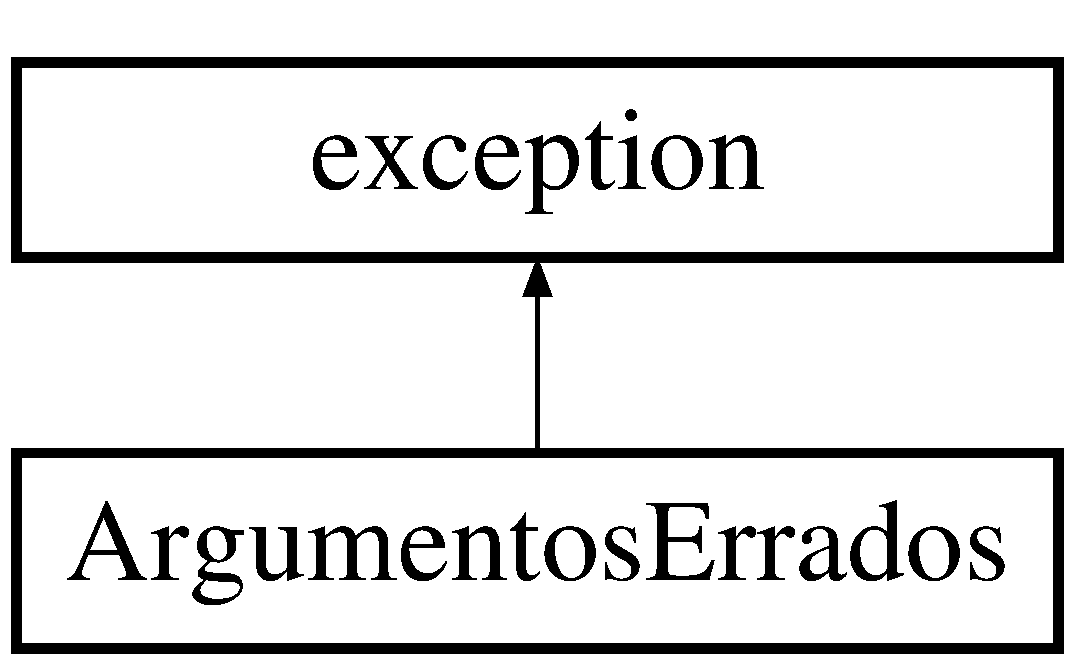
\includegraphics[height=2.000000cm]{classArgumentosErrados}
\end{center}
\end{figure}
\subsection*{Public Member Functions}
\begin{DoxyCompactItemize}
\item 
\mbox{\Hypertarget{classArgumentosErrados_a9d23e10092cd69f8e9fdc94074a24ecf}\label{classArgumentosErrados_a9d23e10092cd69f8e9fdc94074a24ecf}} 
const char $\ast$ {\bfseries what} ()
\end{DoxyCompactItemize}


\subsection{Detailed Description}
Classe de exceção Argumentos errados. 

Verifica se a string dada pelo usuário é válida ou não. \begin{DoxyReturn}{Returns}
Texto. 
\end{DoxyReturn}


The documentation for this class was generated from the following file\+:\begin{DoxyCompactItemize}
\item 
excecao.\+h\end{DoxyCompactItemize}

\hypertarget{classassassino}{}\section{assassino Class Reference}
\label{classassassino}\index{assassino@{assassino}}
Inheritance diagram for assassino\+:\begin{figure}[H]
\begin{center}
\leavevmode
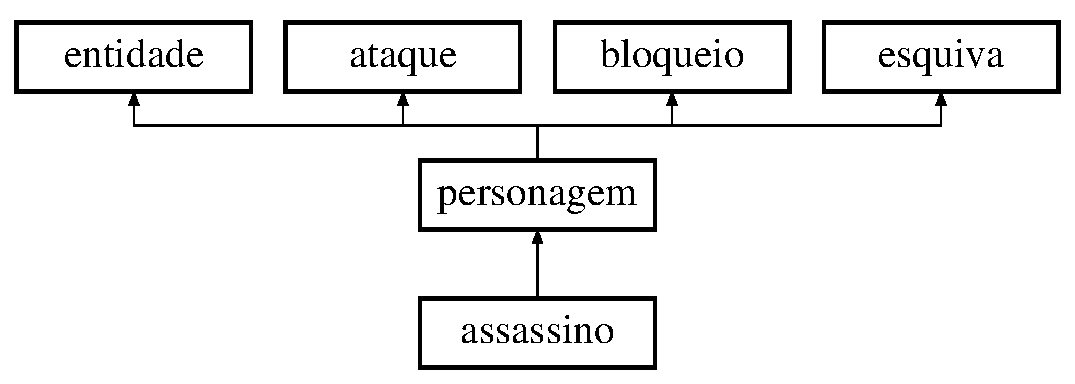
\includegraphics[height=3.000000cm]{classassassino}
\end{center}
\end{figure}
\subsection*{Public Member Functions}
\begin{DoxyCompactItemize}
\item 
\mbox{\hyperlink{classassassino_a107c275bfe816f79279ec3976223974f}{assassino}} (string nome)
\begin{DoxyCompactList}\small\item\em Criação da classe assassino. \end{DoxyCompactList}\item 
int \mbox{\hyperlink{classassassino_a3f46fb60f6617502542fe7377a6499ab}{controle\+Ataque}} (string valor, int arm\+Fisica, int arm\+Runica, int hp)
\begin{DoxyCompactList}\small\item\em Método de controle de ataque. \end{DoxyCompactList}\item 
int \mbox{\hyperlink{classassassino_a02ee2eea7a7f1ca7ca8d1b88e481ab97}{skill\+Um}} (int arm\+Fisica, int arm\+Runica, int hp)
\begin{DoxyCompactList}\small\item\em Método skill\+Um. \end{DoxyCompactList}\item 
int \mbox{\hyperlink{classassassino_acd757ef4b59c18d2aa504a6afa15b107}{skill\+Dois}} (int arm\+Fisica, int arm\+Runica, int hp)
\begin{DoxyCompactList}\small\item\em Método skill dois. \end{DoxyCompactList}\item 
int \mbox{\hyperlink{classassassino_ad13d3c24ad8f2f3e0c7274a1a18a0d39}{skill\+Tres}} (int arm\+Fisica, int arm\+Runica, int hp)
\begin{DoxyCompactList}\small\item\em Método skill\+Tres. \end{DoxyCompactList}\item 
void \mbox{\hyperlink{classassassino_a283e61020246d2bec61fe8e661a412e9}{aplicar\+Debuffs}} ()
\begin{DoxyCompactList}\small\item\em Método aplicar debuffs. \end{DoxyCompactList}\end{DoxyCompactItemize}


\subsection{Constructor \& Destructor Documentation}
\mbox{\Hypertarget{classassassino_a107c275bfe816f79279ec3976223974f}\label{classassassino_a107c275bfe816f79279ec3976223974f}} 
\index{assassino@{assassino}!assassino@{assassino}}
\index{assassino@{assassino}!assassino@{assassino}}
\subsubsection{\texorpdfstring{assassino()}{assassino()}}
{\footnotesize\ttfamily assassino\+::assassino (\begin{DoxyParamCaption}\item[{string}]{Nome }\end{DoxyParamCaption})}



Criação da classe assassino. 

Utilização da classe personagem como base. \begin{DoxyReturn}{Returns}
Objeto assassino. 
\end{DoxyReturn}


\subsection{Member Function Documentation}
\mbox{\Hypertarget{classassassino_a283e61020246d2bec61fe8e661a412e9}\label{classassassino_a283e61020246d2bec61fe8e661a412e9}} 
\index{assassino@{assassino}!aplicar\+Debuffs@{aplicar\+Debuffs}}
\index{aplicar\+Debuffs@{aplicar\+Debuffs}!assassino@{assassino}}
\subsubsection{\texorpdfstring{aplicar\+Debuffs()}{aplicarDebuffs()}}
{\footnotesize\ttfamily void assassino\+::aplicar\+Debuffs (\begin{DoxyParamCaption}{ }\end{DoxyParamCaption})}



Método aplicar debuffs. 

Contabiliza a perca de mana com as skills passiva 2 e 3. \begin{DoxyReturn}{Returns}
void. 
\end{DoxyReturn}
\mbox{\Hypertarget{classassassino_a3f46fb60f6617502542fe7377a6499ab}\label{classassassino_a3f46fb60f6617502542fe7377a6499ab}} 
\index{assassino@{assassino}!controle\+Ataque@{controle\+Ataque}}
\index{controle\+Ataque@{controle\+Ataque}!assassino@{assassino}}
\subsubsection{\texorpdfstring{controle\+Ataque()}{controleAtaque()}}
{\footnotesize\ttfamily int assassino\+::controle\+Ataque (\begin{DoxyParamCaption}\item[{string}]{valor,  }\item[{int}]{arm\+Fisica,  }\item[{int}]{arm\+Runica,  }\item[{int}]{hp }\end{DoxyParamCaption})}



Método de controle de ataque. 

recebe valor do usuário, armadura física, armadura mágica e hp do alvo. \begin{DoxyReturn}{Returns}
dano causado. 
\end{DoxyReturn}
\mbox{\Hypertarget{classassassino_acd757ef4b59c18d2aa504a6afa15b107}\label{classassassino_acd757ef4b59c18d2aa504a6afa15b107}} 
\index{assassino@{assassino}!skill\+Dois@{skill\+Dois}}
\index{skill\+Dois@{skill\+Dois}!assassino@{assassino}}
\subsubsection{\texorpdfstring{skill\+Dois()}{skillDois()}}
{\footnotesize\ttfamily int assassino\+::skill\+Dois (\begin{DoxyParamCaption}\item[{int}]{arm\+Fisica,  }\item[{int}]{arm\+Runica,  }\item[{int}]{hp }\end{DoxyParamCaption})}



Método skill dois. 

Habilita +10 de dano na arma, com custo de 5 de mana por round. \begin{DoxyReturn}{Returns}
Status melhorado ou dano. 
\end{DoxyReturn}
\mbox{\Hypertarget{classassassino_ad13d3c24ad8f2f3e0c7274a1a18a0d39}\label{classassassino_ad13d3c24ad8f2f3e0c7274a1a18a0d39}} 
\index{assassino@{assassino}!skill\+Tres@{skill\+Tres}}
\index{skill\+Tres@{skill\+Tres}!assassino@{assassino}}
\subsubsection{\texorpdfstring{skill\+Tres()}{skillTres()}}
{\footnotesize\ttfamily int assassino\+::skill\+Tres (\begin{DoxyParamCaption}\item[{int}]{arm\+Fisica,  }\item[{int}]{arm\+Runica,  }\item[{int}]{hp }\end{DoxyParamCaption})}



Método skill\+Tres. 

Seta esquiva como 100 ao custo de perder 20 de mana continuamente. \begin{DoxyReturn}{Returns}
Set\+Esquiva ou dano. 
\end{DoxyReturn}
\mbox{\Hypertarget{classassassino_a02ee2eea7a7f1ca7ca8d1b88e481ab97}\label{classassassino_a02ee2eea7a7f1ca7ca8d1b88e481ab97}} 
\index{assassino@{assassino}!skill\+Um@{skill\+Um}}
\index{skill\+Um@{skill\+Um}!assassino@{assassino}}
\subsubsection{\texorpdfstring{skill\+Um()}{skillUm()}}
{\footnotesize\ttfamily int assassino\+::skill\+Um (\begin{DoxyParamCaption}\item[{int}]{arm\+Fisica,  }\item[{int}]{arm\+Runica,  }\item[{int}]{hp }\end{DoxyParamCaption})}



Método skill\+Um. 

Dobra o dano físico causado a custo de 5 de mana. \begin{DoxyReturn}{Returns}
Dano causado. 
\end{DoxyReturn}


The documentation for this class was generated from the following files\+:\begin{DoxyCompactItemize}
\item 
assassino.\+h\item 
assassino.\+cpp\end{DoxyCompactItemize}

\hypertarget{classataque}{}\section{ataque Class Reference}
\label{classataque}\index{ataque@{ataque}}
Inheritance diagram for ataque\+:\begin{figure}[H]
\begin{center}
\leavevmode
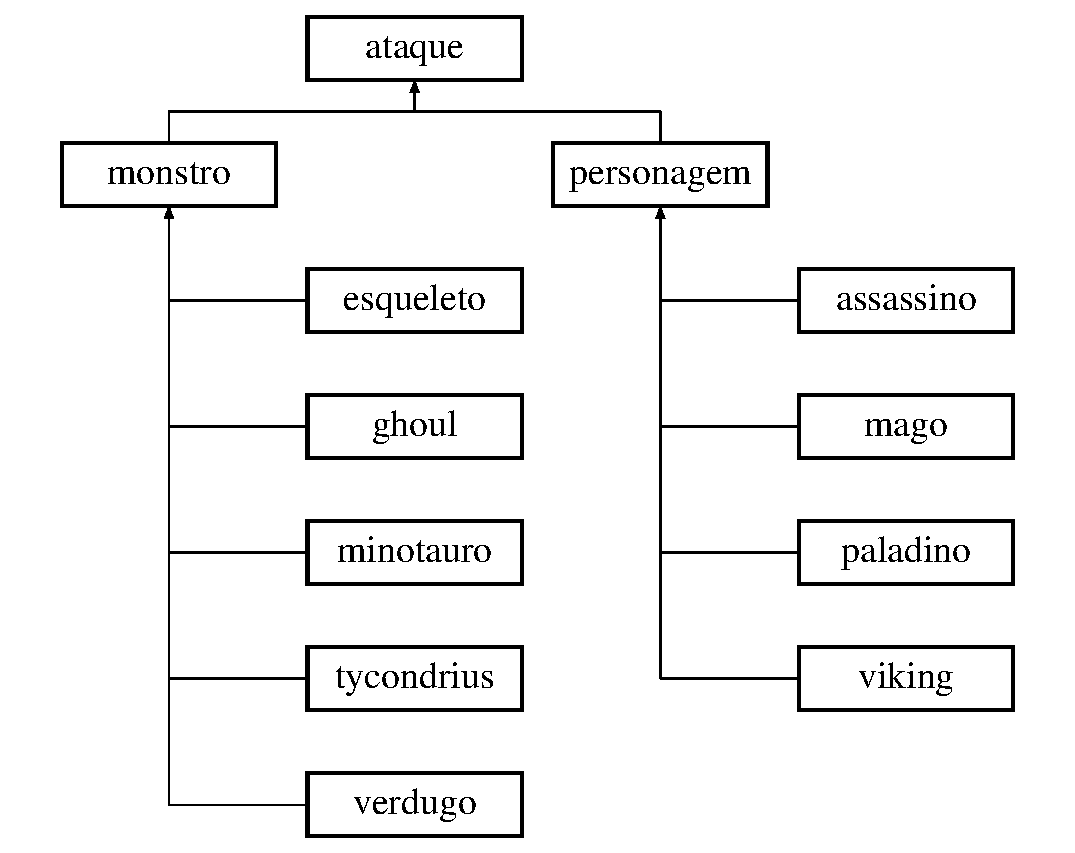
\includegraphics[height=7.000000cm]{classataque}
\end{center}
\end{figure}
\subsection*{Public Member Functions}
\begin{DoxyCompactItemize}
\item 
\mbox{\hyperlink{classataque_aa743f532bf31ac7541ce0963a838021c}{ataque}} (int valor)
\begin{DoxyCompactList}\small\item\em Criação do objeto ataque. \end{DoxyCompactList}\item 
int \mbox{\hyperlink{classataque_a431a441a9a11d651dba80b83f6a9a980}{realizar\+Dano}} (int \mbox{\hyperlink{classbloqueio}{bloqueio}})
\begin{DoxyCompactList}\small\item\em Método de realizar dano. \end{DoxyCompactList}\item 
int \mbox{\hyperlink{classataque_ae21cc54ec16f06614dedddb18d861fda}{get\+Valor\+Ataque}} ()
\begin{DoxyCompactList}\small\item\em Método get para obtênção do valor de ataque. \end{DoxyCompactList}\item 
int \mbox{\hyperlink{classataque_abbd99389ed66a4fdbfe994c3f1a102ec}{get\+Valor\+Dano}} ()
\begin{DoxyCompactList}\small\item\em Método get para obtênção do valor do dano. \end{DoxyCompactList}\item 
void \mbox{\hyperlink{classataque_a398d632b079837ca60dc838671d4614e}{set\+Valor\+Ataque}} (int x)
\begin{DoxyCompactList}\small\item\em Método set para o valor de ataque. \end{DoxyCompactList}\end{DoxyCompactItemize}


\subsection{Constructor \& Destructor Documentation}
\mbox{\Hypertarget{classataque_aa743f532bf31ac7541ce0963a838021c}\label{classataque_aa743f532bf31ac7541ce0963a838021c}} 
\index{ataque@{ataque}!ataque@{ataque}}
\index{ataque@{ataque}!ataque@{ataque}}
\subsubsection{\texorpdfstring{ataque()}{ataque()}}
{\footnotesize\ttfamily ataque\+::ataque (\begin{DoxyParamCaption}\item[{int}]{valor }\end{DoxyParamCaption})}



Criação do objeto ataque. 

Atribui-\/se valor de ataque conforme informado. \begin{DoxyReturn}{Returns}
Objeto ataque. 
\end{DoxyReturn}


\subsection{Member Function Documentation}
\mbox{\Hypertarget{classataque_ae21cc54ec16f06614dedddb18d861fda}\label{classataque_ae21cc54ec16f06614dedddb18d861fda}} 
\index{ataque@{ataque}!get\+Valor\+Ataque@{get\+Valor\+Ataque}}
\index{get\+Valor\+Ataque@{get\+Valor\+Ataque}!ataque@{ataque}}
\subsubsection{\texorpdfstring{get\+Valor\+Ataque()}{getValorAtaque()}}
{\footnotesize\ttfamily int ataque\+::get\+Valor\+Ataque (\begin{DoxyParamCaption}{ }\end{DoxyParamCaption})}



Método get para obtênção do valor de ataque. 

\begin{DoxyReturn}{Returns}
Valor de ataque. 
\end{DoxyReturn}
\mbox{\Hypertarget{classataque_abbd99389ed66a4fdbfe994c3f1a102ec}\label{classataque_abbd99389ed66a4fdbfe994c3f1a102ec}} 
\index{ataque@{ataque}!get\+Valor\+Dano@{get\+Valor\+Dano}}
\index{get\+Valor\+Dano@{get\+Valor\+Dano}!ataque@{ataque}}
\subsubsection{\texorpdfstring{get\+Valor\+Dano()}{getValorDano()}}
{\footnotesize\ttfamily int ataque\+::get\+Valor\+Dano (\begin{DoxyParamCaption}{ }\end{DoxyParamCaption})}



Método get para obtênção do valor do dano. 

\begin{DoxyReturn}{Returns}
Valor do dano. 
\end{DoxyReturn}
\mbox{\Hypertarget{classataque_a431a441a9a11d651dba80b83f6a9a980}\label{classataque_a431a441a9a11d651dba80b83f6a9a980}} 
\index{ataque@{ataque}!realizar\+Dano@{realizar\+Dano}}
\index{realizar\+Dano@{realizar\+Dano}!ataque@{ataque}}
\subsubsection{\texorpdfstring{realizar\+Dano()}{realizarDano()}}
{\footnotesize\ttfamily int ataque\+::realizar\+Dano (\begin{DoxyParamCaption}\item[{int}]{bloqueio }\end{DoxyParamCaption})}



Método de realizar dano. 

Calcula o dano baseaso no valor informado. \begin{DoxyReturn}{Returns}
Valor do dano. 
\end{DoxyReturn}
\mbox{\Hypertarget{classataque_a398d632b079837ca60dc838671d4614e}\label{classataque_a398d632b079837ca60dc838671d4614e}} 
\index{ataque@{ataque}!set\+Valor\+Ataque@{set\+Valor\+Ataque}}
\index{set\+Valor\+Ataque@{set\+Valor\+Ataque}!ataque@{ataque}}
\subsubsection{\texorpdfstring{set\+Valor\+Ataque()}{setValorAtaque()}}
{\footnotesize\ttfamily void ataque\+::set\+Valor\+Ataque (\begin{DoxyParamCaption}\item[{int}]{x }\end{DoxyParamCaption})}



Método set para o valor de ataque. 

\begin{DoxyReturn}{Returns}
void 
\end{DoxyReturn}


The documentation for this class was generated from the following files\+:\begin{DoxyCompactItemize}
\item 
ataque.\+h\item 
ataque.\+cpp\end{DoxyCompactItemize}

\hypertarget{classbloqueio}{}\section{bloqueio Class Reference}
\label{classbloqueio}\index{bloqueio@{bloqueio}}
Inheritance diagram for bloqueio\+:\begin{figure}[H]
\begin{center}
\leavevmode
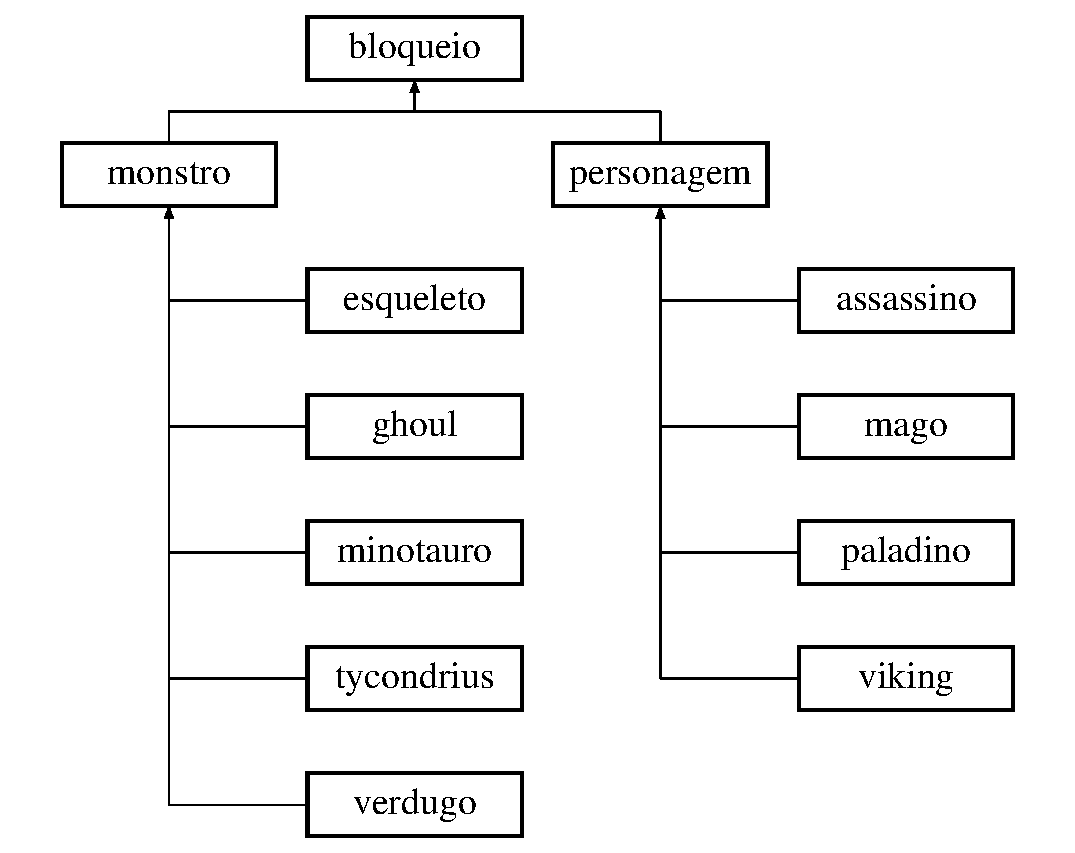
\includegraphics[height=7.000000cm]{classbloqueio}
\end{center}
\end{figure}
\subsection*{Public Member Functions}
\begin{DoxyCompactItemize}
\item 
\mbox{\hyperlink{classbloqueio_aa43a8bb2b16af5907e8e78a54a432afe}{bloqueio}} (int arm\+Fisica, int arm\+Runica)
\begin{DoxyCompactList}\small\item\em Criação do objeto bloqueio. \end{DoxyCompactList}\item 
int \mbox{\hyperlink{classbloqueio_a1d06f5be69ab5f74f983fe7de1efe41c}{get\+Armadura\+Runica}} ()
\begin{DoxyCompactList}\small\item\em Método get armadura rûnica. \end{DoxyCompactList}\item 
int \mbox{\hyperlink{classbloqueio_a7bdccc95284f88b2c30fe9b35bc26a2b}{get\+Armadura\+Fisica}} ()
\begin{DoxyCompactList}\small\item\em Método get armadura física. \end{DoxyCompactList}\item 
void \mbox{\hyperlink{classbloqueio_a93d5e345503601ea3c06367e5ab0797b}{set\+Armadura\+Runica}} (int x)
\begin{DoxyCompactList}\small\item\em Método set armadura rûnica. \end{DoxyCompactList}\item 
void \mbox{\hyperlink{classbloqueio_ab47b5ba74cd295c9998ba042773d9814}{set\+Armadura\+Fisica}} (int y)
\begin{DoxyCompactList}\small\item\em Método set armadura física. \end{DoxyCompactList}\end{DoxyCompactItemize}


\subsection{Constructor \& Destructor Documentation}
\mbox{\Hypertarget{classbloqueio_aa43a8bb2b16af5907e8e78a54a432afe}\label{classbloqueio_aa43a8bb2b16af5907e8e78a54a432afe}} 
\index{bloqueio@{bloqueio}!bloqueio@{bloqueio}}
\index{bloqueio@{bloqueio}!bloqueio@{bloqueio}}
\subsubsection{\texorpdfstring{bloqueio()}{bloqueio()}}
{\footnotesize\ttfamily bloqueio\+::bloqueio (\begin{DoxyParamCaption}\item[{int}]{arm\+Fisica,  }\item[{int}]{arm\+Runica }\end{DoxyParamCaption})}



Criação do objeto bloqueio. 

Recebe a armadura rûnica e física para construção do objeto. \begin{DoxyReturn}{Returns}
Objeto bloqueio. 
\end{DoxyReturn}


\subsection{Member Function Documentation}
\mbox{\Hypertarget{classbloqueio_a7bdccc95284f88b2c30fe9b35bc26a2b}\label{classbloqueio_a7bdccc95284f88b2c30fe9b35bc26a2b}} 
\index{bloqueio@{bloqueio}!get\+Armadura\+Fisica@{get\+Armadura\+Fisica}}
\index{get\+Armadura\+Fisica@{get\+Armadura\+Fisica}!bloqueio@{bloqueio}}
\subsubsection{\texorpdfstring{get\+Armadura\+Fisica()}{getArmaduraFisica()}}
{\footnotesize\ttfamily int bloqueio\+::get\+Armadura\+Fisica (\begin{DoxyParamCaption}{ }\end{DoxyParamCaption})}



Método get armadura física. 

\begin{DoxyReturn}{Returns}
Armadura física. 
\end{DoxyReturn}
\mbox{\Hypertarget{classbloqueio_a1d06f5be69ab5f74f983fe7de1efe41c}\label{classbloqueio_a1d06f5be69ab5f74f983fe7de1efe41c}} 
\index{bloqueio@{bloqueio}!get\+Armadura\+Runica@{get\+Armadura\+Runica}}
\index{get\+Armadura\+Runica@{get\+Armadura\+Runica}!bloqueio@{bloqueio}}
\subsubsection{\texorpdfstring{get\+Armadura\+Runica()}{getArmaduraRunica()}}
{\footnotesize\ttfamily int bloqueio\+::get\+Armadura\+Runica (\begin{DoxyParamCaption}{ }\end{DoxyParamCaption})}



Método get armadura rûnica. 

\begin{DoxyReturn}{Returns}
Armadura rûnica. 
\end{DoxyReturn}
\mbox{\Hypertarget{classbloqueio_ab47b5ba74cd295c9998ba042773d9814}\label{classbloqueio_ab47b5ba74cd295c9998ba042773d9814}} 
\index{bloqueio@{bloqueio}!set\+Armadura\+Fisica@{set\+Armadura\+Fisica}}
\index{set\+Armadura\+Fisica@{set\+Armadura\+Fisica}!bloqueio@{bloqueio}}
\subsubsection{\texorpdfstring{set\+Armadura\+Fisica()}{setArmaduraFisica()}}
{\footnotesize\ttfamily void bloqueio\+::set\+Armadura\+Fisica (\begin{DoxyParamCaption}\item[{int}]{y }\end{DoxyParamCaption})}



Método set armadura física. 

\begin{DoxyReturn}{Returns}
void. 
\end{DoxyReturn}
\mbox{\Hypertarget{classbloqueio_a93d5e345503601ea3c06367e5ab0797b}\label{classbloqueio_a93d5e345503601ea3c06367e5ab0797b}} 
\index{bloqueio@{bloqueio}!set\+Armadura\+Runica@{set\+Armadura\+Runica}}
\index{set\+Armadura\+Runica@{set\+Armadura\+Runica}!bloqueio@{bloqueio}}
\subsubsection{\texorpdfstring{set\+Armadura\+Runica()}{setArmaduraRunica()}}
{\footnotesize\ttfamily void bloqueio\+::set\+Armadura\+Runica (\begin{DoxyParamCaption}\item[{int}]{x }\end{DoxyParamCaption})}



Método set armadura rûnica. 

\begin{DoxyReturn}{Returns}
void. 
\end{DoxyReturn}


The documentation for this class was generated from the following files\+:\begin{DoxyCompactItemize}
\item 
bloqueio.\+h\item 
bloqueio.\+cpp\end{DoxyCompactItemize}

\hypertarget{classdado}{}\section{dado Class Reference}
\label{classdado}\index{dado@{dado}}
\subsection*{Public Member Functions}
\begin{DoxyCompactItemize}
\item 
\mbox{\hyperlink{classdado_a65c1404cb80eb753215830d2f176f334}{dado}} (int Valor)
\begin{DoxyCompactList}\small\item\em Criação do objeto Dado. \end{DoxyCompactList}\item 
int \mbox{\hyperlink{classdado_a768c4cc0bfb5f9d4b7dbdeb2fb11c5fa}{Jogar}} ()
\begin{DoxyCompactList}\small\item\em Método jogar. \end{DoxyCompactList}\item 
int \mbox{\hyperlink{classdado_a94a38beee28359ee6005889d5d32e754}{get\+Valor}} ()
\begin{DoxyCompactList}\small\item\em Método get do valor. \end{DoxyCompactList}\end{DoxyCompactItemize}


\subsection{Constructor \& Destructor Documentation}
\mbox{\Hypertarget{classdado_a65c1404cb80eb753215830d2f176f334}\label{classdado_a65c1404cb80eb753215830d2f176f334}} 
\index{dado@{dado}!dado@{dado}}
\index{dado@{dado}!dado@{dado}}
\subsubsection{\texorpdfstring{dado()}{dado()}}
{\footnotesize\ttfamily dado\+::dado (\begin{DoxyParamCaption}\item[{int}]{Valor }\end{DoxyParamCaption})}



Criação do objeto Dado. 

Recebe um valor e estipula o sorteio de 1 até esse valor. \begin{DoxyReturn}{Returns}
Objeto dado. 
\end{DoxyReturn}


\subsection{Member Function Documentation}
\mbox{\Hypertarget{classdado_a94a38beee28359ee6005889d5d32e754}\label{classdado_a94a38beee28359ee6005889d5d32e754}} 
\index{dado@{dado}!get\+Valor@{get\+Valor}}
\index{get\+Valor@{get\+Valor}!dado@{dado}}
\subsubsection{\texorpdfstring{get\+Valor()}{getValor()}}
{\footnotesize\ttfamily int dado\+::get\+Valor (\begin{DoxyParamCaption}{ }\end{DoxyParamCaption})}



Método get do valor. 

\begin{DoxyReturn}{Returns}
Valor do dado. 
\end{DoxyReturn}
\mbox{\Hypertarget{classdado_a768c4cc0bfb5f9d4b7dbdeb2fb11c5fa}\label{classdado_a768c4cc0bfb5f9d4b7dbdeb2fb11c5fa}} 
\index{dado@{dado}!Jogar@{Jogar}}
\index{Jogar@{Jogar}!dado@{dado}}
\subsubsection{\texorpdfstring{Jogar()}{Jogar()}}
{\footnotesize\ttfamily int dado\+::\+Jogar (\begin{DoxyParamCaption}{ }\end{DoxyParamCaption})}



Método jogar. 

Baseado no valor informado faz se um sorteio pseudo aleatório. \begin{DoxyReturn}{Returns}
Valor do sorteio. 
\end{DoxyReturn}


The documentation for this class was generated from the following files\+:\begin{DoxyCompactItemize}
\item 
dado.\+h\item 
dado.\+cpp\end{DoxyCompactItemize}

\hypertarget{classentidade}{}\section{entidade Class Reference}
\label{classentidade}\index{entidade@{entidade}}
Inheritance diagram for entidade\+:\begin{figure}[H]
\begin{center}
\leavevmode
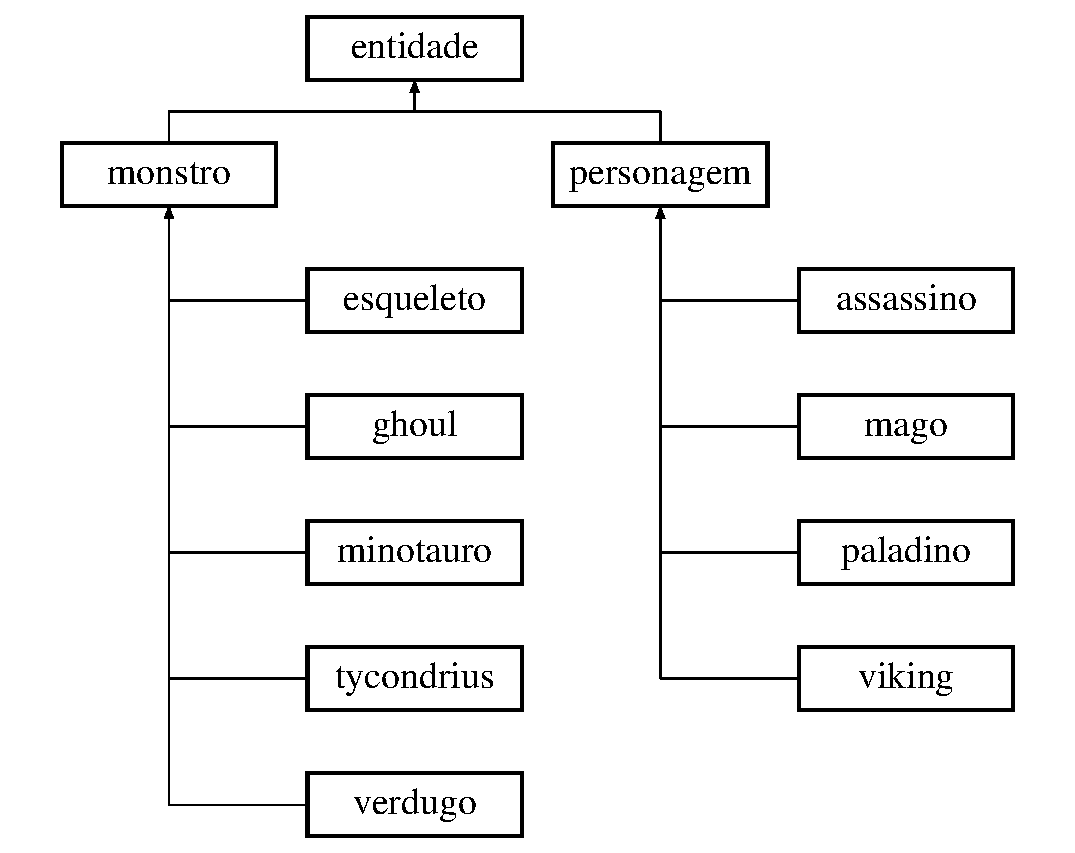
\includegraphics[height=7.000000cm]{classentidade}
\end{center}
\end{figure}
\subsection*{Public Member Functions}
\begin{DoxyCompactItemize}
\item 
\mbox{\hyperlink{classentidade_a1ae08f868dbdfaa1e85a6799b074d769}{entidade}} (int hp, int mana)
\begin{DoxyCompactList}\small\item\em Criação do objeto entidade. \end{DoxyCompactList}\item 
int \mbox{\hyperlink{classentidade_a1cbf074af4a67d31091265e677502b8e}{get\+HP}} ()
\begin{DoxyCompactList}\small\item\em Método get do hp. \end{DoxyCompactList}\item 
int \mbox{\hyperlink{classentidade_a0fa69d3b04a023da3d474e18619d27f7}{get\+Mana}} ()
\begin{DoxyCompactList}\small\item\em Método get da mana. \end{DoxyCompactList}\item 
void \mbox{\hyperlink{classentidade_abbd3175dda4fa70fd2ef4c7bf8dd6c2e}{debitar\+HP}} (int valor)
\begin{DoxyCompactList}\small\item\em Método debitar hp. \end{DoxyCompactList}\item 
void \mbox{\hyperlink{classentidade_a16d5689ead06cec1a6ad52dde8989e96}{debitar\+Mana}} (int valor)
\begin{DoxyCompactList}\small\item\em Método debitar mana. \end{DoxyCompactList}\item 
void \mbox{\hyperlink{classentidade_ae30252d3e3b769a7b56d994552bb2856}{set\+HP}} (int valor)
\begin{DoxyCompactList}\small\item\em Método set hp. \end{DoxyCompactList}\item 
void \mbox{\hyperlink{classentidade_acc3d424b1cdad2cc19c03cc0bff4cce6}{set\+Mana}} (int valor)
\begin{DoxyCompactList}\small\item\em Método set mana. \end{DoxyCompactList}\end{DoxyCompactItemize}


\subsection{Constructor \& Destructor Documentation}
\mbox{\Hypertarget{classentidade_a1ae08f868dbdfaa1e85a6799b074d769}\label{classentidade_a1ae08f868dbdfaa1e85a6799b074d769}} 
\index{entidade@{entidade}!entidade@{entidade}}
\index{entidade@{entidade}!entidade@{entidade}}
\subsubsection{\texorpdfstring{entidade()}{entidade()}}
{\footnotesize\ttfamily entidade\+::entidade (\begin{DoxyParamCaption}\item[{int}]{hp,  }\item[{int}]{mana }\end{DoxyParamCaption})}



Criação do objeto entidade. 

Recebe os valores de hp e mana da entidade. \begin{DoxyReturn}{Returns}
Objeto entidade. 
\end{DoxyReturn}


\subsection{Member Function Documentation}
\mbox{\Hypertarget{classentidade_abbd3175dda4fa70fd2ef4c7bf8dd6c2e}\label{classentidade_abbd3175dda4fa70fd2ef4c7bf8dd6c2e}} 
\index{entidade@{entidade}!debitar\+HP@{debitar\+HP}}
\index{debitar\+HP@{debitar\+HP}!entidade@{entidade}}
\subsubsection{\texorpdfstring{debitar\+H\+P()}{debitarHP()}}
{\footnotesize\ttfamily void entidade\+::debitar\+HP (\begin{DoxyParamCaption}\item[{int}]{valor }\end{DoxyParamCaption})}



Método debitar hp. 

Reduz o valor do hp da entidade baseado no valor informado. \begin{DoxyReturn}{Returns}
void. 
\end{DoxyReturn}
\mbox{\Hypertarget{classentidade_a16d5689ead06cec1a6ad52dde8989e96}\label{classentidade_a16d5689ead06cec1a6ad52dde8989e96}} 
\index{entidade@{entidade}!debitar\+Mana@{debitar\+Mana}}
\index{debitar\+Mana@{debitar\+Mana}!entidade@{entidade}}
\subsubsection{\texorpdfstring{debitar\+Mana()}{debitarMana()}}
{\footnotesize\ttfamily void entidade\+::debitar\+Mana (\begin{DoxyParamCaption}\item[{int}]{valor }\end{DoxyParamCaption})}



Método debitar mana. 

Reduz o valor da mana da entidade baseado no valor informado. \begin{DoxyReturn}{Returns}
void. 
\end{DoxyReturn}
\mbox{\Hypertarget{classentidade_a1cbf074af4a67d31091265e677502b8e}\label{classentidade_a1cbf074af4a67d31091265e677502b8e}} 
\index{entidade@{entidade}!get\+HP@{get\+HP}}
\index{get\+HP@{get\+HP}!entidade@{entidade}}
\subsubsection{\texorpdfstring{get\+H\+P()}{getHP()}}
{\footnotesize\ttfamily int entidade\+::get\+HP (\begin{DoxyParamCaption}{ }\end{DoxyParamCaption})}



Método get do hp. 

\begin{DoxyReturn}{Returns}
hp da entidade. 
\end{DoxyReturn}
\mbox{\Hypertarget{classentidade_a0fa69d3b04a023da3d474e18619d27f7}\label{classentidade_a0fa69d3b04a023da3d474e18619d27f7}} 
\index{entidade@{entidade}!get\+Mana@{get\+Mana}}
\index{get\+Mana@{get\+Mana}!entidade@{entidade}}
\subsubsection{\texorpdfstring{get\+Mana()}{getMana()}}
{\footnotesize\ttfamily int entidade\+::get\+Mana (\begin{DoxyParamCaption}{ }\end{DoxyParamCaption})}



Método get da mana. 

\begin{DoxyReturn}{Returns}
mana da entidade. 
\end{DoxyReturn}
\mbox{\Hypertarget{classentidade_ae30252d3e3b769a7b56d994552bb2856}\label{classentidade_ae30252d3e3b769a7b56d994552bb2856}} 
\index{entidade@{entidade}!set\+HP@{set\+HP}}
\index{set\+HP@{set\+HP}!entidade@{entidade}}
\subsubsection{\texorpdfstring{set\+H\+P()}{setHP()}}
{\footnotesize\ttfamily void entidade\+::set\+HP (\begin{DoxyParamCaption}\item[{int}]{valor }\end{DoxyParamCaption})}



Método set hp. 

\begin{DoxyReturn}{Returns}

\end{DoxyReturn}
\mbox{\Hypertarget{classentidade_acc3d424b1cdad2cc19c03cc0bff4cce6}\label{classentidade_acc3d424b1cdad2cc19c03cc0bff4cce6}} 
\index{entidade@{entidade}!set\+Mana@{set\+Mana}}
\index{set\+Mana@{set\+Mana}!entidade@{entidade}}
\subsubsection{\texorpdfstring{set\+Mana()}{setMana()}}
{\footnotesize\ttfamily void entidade\+::set\+Mana (\begin{DoxyParamCaption}\item[{int}]{valor }\end{DoxyParamCaption})}



Método set mana. 

\begin{DoxyReturn}{Returns}

\end{DoxyReturn}


The documentation for this class was generated from the following files\+:\begin{DoxyCompactItemize}
\item 
entidade.\+h\item 
entidade.\+cpp\end{DoxyCompactItemize}

\hypertarget{classesqueleto}{}\section{esqueleto Class Reference}
\label{classesqueleto}\index{esqueleto@{esqueleto}}
Inheritance diagram for esqueleto\+:\begin{figure}[H]
\begin{center}
\leavevmode
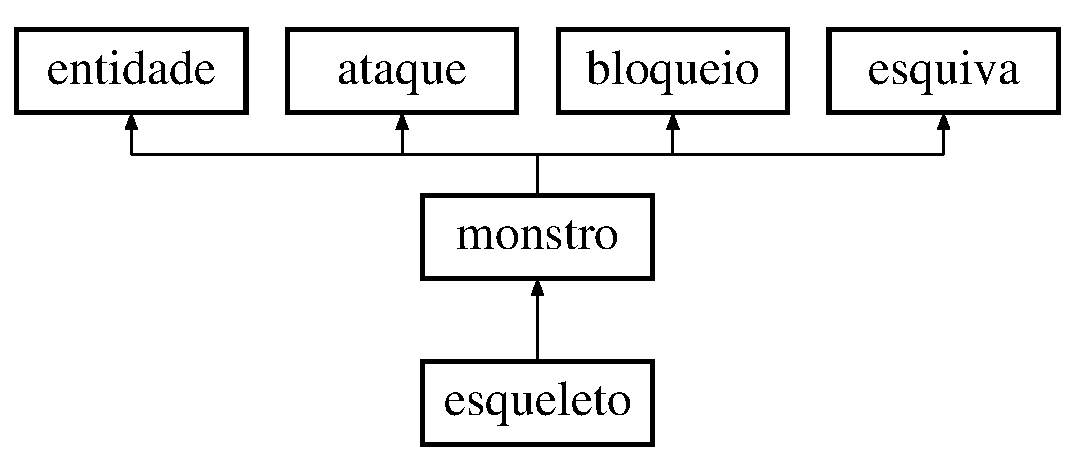
\includegraphics[height=3.000000cm]{classesqueleto}
\end{center}
\end{figure}
\subsection*{Public Member Functions}
\begin{DoxyCompactItemize}
\item 
\mbox{\hyperlink{classesqueleto_a78b38d1c397903f66b1c527fd6dfef97}{esqueleto}} ()
\begin{DoxyCompactList}\small\item\em Criação da classe esqueleto. \end{DoxyCompactList}\end{DoxyCompactItemize}


\subsection{Constructor \& Destructor Documentation}
\mbox{\Hypertarget{classesqueleto_a78b38d1c397903f66b1c527fd6dfef97}\label{classesqueleto_a78b38d1c397903f66b1c527fd6dfef97}} 
\index{esqueleto@{esqueleto}!esqueleto@{esqueleto}}
\index{esqueleto@{esqueleto}!esqueleto@{esqueleto}}
\subsubsection{\texorpdfstring{esqueleto()}{esqueleto()}}
{\footnotesize\ttfamily esqueleto\+::esqueleto (\begin{DoxyParamCaption}{ }\end{DoxyParamCaption})}



Criação da classe esqueleto. 

Utilização da classe monstro como base. \begin{DoxyReturn}{Returns}
Objeto esqueleto. 
\end{DoxyReturn}


The documentation for this class was generated from the following files\+:\begin{DoxyCompactItemize}
\item 
esqueleto.\+h\item 
esqueleto.\+cpp\end{DoxyCompactItemize}

\hypertarget{classesquiva}{}\section{esquiva Class Reference}
\label{classesquiva}\index{esquiva@{esquiva}}
Inheritance diagram for esquiva\+:\begin{figure}[H]
\begin{center}
\leavevmode
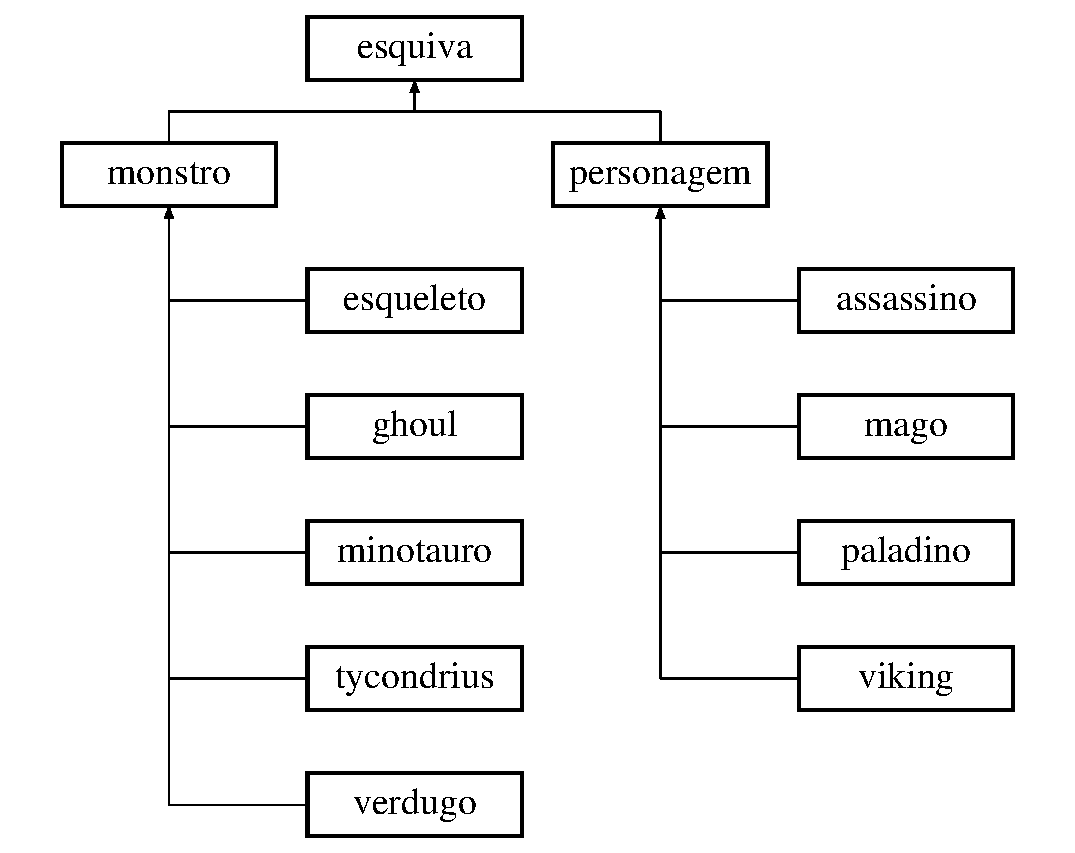
\includegraphics[height=7.000000cm]{classesquiva}
\end{center}
\end{figure}
\subsection*{Public Member Functions}
\begin{DoxyCompactItemize}
\item 
\mbox{\hyperlink{classesquiva_af611f7fe8c69b85f58e1d3eb41af611a}{esquiva}} (int valor)
\begin{DoxyCompactList}\small\item\em Criação do objeto esquiva. \end{DoxyCompactList}\item 
int \mbox{\hyperlink{classesquiva_a0defb7805011650e62e3e8c1cf362a53}{get\+Esquiva}} ()
\begin{DoxyCompactList}\small\item\em Método get de esquiva. \end{DoxyCompactList}\item 
void \mbox{\hyperlink{classesquiva_a782b543697b0578e0f8efaed5b631209}{set\+Esquiva}} (int valor)
\begin{DoxyCompactList}\small\item\em Método set de esquiva. \end{DoxyCompactList}\item 
bool \mbox{\hyperlink{classesquiva_a52c90c2a26c3d27e1549e5469c49c1bb}{esquivar}} ()
\begin{DoxyCompactList}\small\item\em Método esquivar. \end{DoxyCompactList}\end{DoxyCompactItemize}


\subsection{Constructor \& Destructor Documentation}
\mbox{\Hypertarget{classesquiva_af611f7fe8c69b85f58e1d3eb41af611a}\label{classesquiva_af611f7fe8c69b85f58e1d3eb41af611a}} 
\index{esquiva@{esquiva}!esquiva@{esquiva}}
\index{esquiva@{esquiva}!esquiva@{esquiva}}
\subsubsection{\texorpdfstring{esquiva()}{esquiva()}}
{\footnotesize\ttfamily esquiva\+::esquiva (\begin{DoxyParamCaption}\item[{int}]{valor }\end{DoxyParamCaption})}



Criação do objeto esquiva. 

Recebe o valor de esquiva e cria-\/se um dado D100. \begin{DoxyReturn}{Returns}
Objeto esquiva. 
\end{DoxyReturn}


\subsection{Member Function Documentation}
\mbox{\Hypertarget{classesquiva_a52c90c2a26c3d27e1549e5469c49c1bb}\label{classesquiva_a52c90c2a26c3d27e1549e5469c49c1bb}} 
\index{esquiva@{esquiva}!esquivar@{esquivar}}
\index{esquivar@{esquivar}!esquiva@{esquiva}}
\subsubsection{\texorpdfstring{esquivar()}{esquivar()}}
{\footnotesize\ttfamily bool esquiva\+::esquivar (\begin{DoxyParamCaption}{ }\end{DoxyParamCaption})}



Método esquivar. 

Joga-\/se um dado D100 e baseado no rate de esquiva determina se o alvo vai ou não se esquivar. \begin{DoxyReturn}{Returns}
Bool valor. 
\end{DoxyReturn}
\mbox{\Hypertarget{classesquiva_a0defb7805011650e62e3e8c1cf362a53}\label{classesquiva_a0defb7805011650e62e3e8c1cf362a53}} 
\index{esquiva@{esquiva}!get\+Esquiva@{get\+Esquiva}}
\index{get\+Esquiva@{get\+Esquiva}!esquiva@{esquiva}}
\subsubsection{\texorpdfstring{get\+Esquiva()}{getEsquiva()}}
{\footnotesize\ttfamily int esquiva\+::get\+Esquiva (\begin{DoxyParamCaption}{ }\end{DoxyParamCaption})}



Método get de esquiva. 

\begin{DoxyReturn}{Returns}
rate\+Esquiva. 
\end{DoxyReturn}
\mbox{\Hypertarget{classesquiva_a782b543697b0578e0f8efaed5b631209}\label{classesquiva_a782b543697b0578e0f8efaed5b631209}} 
\index{esquiva@{esquiva}!set\+Esquiva@{set\+Esquiva}}
\index{set\+Esquiva@{set\+Esquiva}!esquiva@{esquiva}}
\subsubsection{\texorpdfstring{set\+Esquiva()}{setEsquiva()}}
{\footnotesize\ttfamily void esquiva\+::set\+Esquiva (\begin{DoxyParamCaption}\item[{int}]{valor }\end{DoxyParamCaption})}



Método set de esquiva. 

\begin{DoxyReturn}{Returns}
void. 
\end{DoxyReturn}


The documentation for this class was generated from the following files\+:\begin{DoxyCompactItemize}
\item 
esquiva.\+h\item 
esquiva.\+cpp\end{DoxyCompactItemize}

\hypertarget{classfases}{}\section{fases Class Reference}
\label{classfases}\index{fases@{fases}}
\subsection*{Public Member Functions}
\begin{DoxyCompactItemize}
\item 
\mbox{\hyperlink{classfases_a39d5b42a40a958d25411c51cb2b0959c}{fases}} ()
\begin{DoxyCompactList}\small\item\em Construção da classe Fases. \end{DoxyCompactList}\item 
void \mbox{\hyperlink{classfases_a89059232b76460277f9846fc6d66488c}{fase\+Um}} ()
\begin{DoxyCompactList}\small\item\em Método fase\+Um. \end{DoxyCompactList}\item 
void \mbox{\hyperlink{classfases_a2f19632bd94eacd6c5437a2774bc529f}{fase\+Dois}} ()
\begin{DoxyCompactList}\small\item\em Método fase\+Dois. \end{DoxyCompactList}\item 
void \mbox{\hyperlink{classfases_a05138769008d5c7d1b548916ecfa9f34}{fase\+Tres}} ()
\begin{DoxyCompactList}\small\item\em Método fase\+Tres. \end{DoxyCompactList}\item 
void \mbox{\hyperlink{classfases_af33d3aefdf442b1ea726645b0c946d78}{fase\+Quatro}} ()
\begin{DoxyCompactList}\small\item\em Método fase\+Quatro. \end{DoxyCompactList}\item 
void \mbox{\hyperlink{classfases_aa05ea0c25d2c70ee022f56f02003b4b5}{End\+Game}} ()
<<<<<<< HEAD
\begin{DoxyCompactList}\small\item\em Método End\+Game. \end{DoxyCompactList}\item 
bool \mbox{\hyperlink{classfases_aedbb30c3e8ad0b50e96561029aecdf4a}{get\+End\+Game}} ()
\begin{DoxyCompactList}\small\item\em Método get End Game. \end{DoxyCompactList}\end{DoxyCompactItemize}
\subsection*{Friends}
\begin{DoxyCompactItemize}
\item 
istream \& \mbox{\hyperlink{classfases_a24bc7622c7828e59917da245c41920d8}{operator$>$$>$}} (istream \&i, \mbox{\hyperlink{classfases}{fases}} \&t)
\begin{DoxyCompactList}\small\item\em Sobrecarga do operado $>$$>$. \end{DoxyCompactList}\item 
ostream \& \mbox{\hyperlink{classfases_a918b9b50f8716407ea46bdfbf5848271}{operator$<$$<$}} (ostream \&o, \mbox{\hyperlink{classfases}{fases}} \&t)
\begin{DoxyCompactList}\small\item\em Sobrecarga do operado $<$$<$. \end{DoxyCompactList}\end{DoxyCompactItemize}
=======
\begin{DoxyCompactList}\small\item\em Método End\+Game. \end{DoxyCompactList}\end{DoxyCompactItemize}
>>>>>>> 0546f94c50e08ebf892bc8350edb40cb6ecd7634


\subsection{Constructor \& Destructor Documentation}
\mbox{\Hypertarget{classfases_a39d5b42a40a958d25411c51cb2b0959c}\label{classfases_a39d5b42a40a958d25411c51cb2b0959c}} 
\index{fases@{fases}!fases@{fases}}
\index{fases@{fases}!fases@{fases}}
\subsubsection{\texorpdfstring{fases()}{fases()}}
{\footnotesize\ttfamily fases\+::fases (\begin{DoxyParamCaption}{ }\end{DoxyParamCaption})}



Construção da classe Fases. 

Classe baseada na construção do jogo. \begin{DoxyReturn}{Returns}
Objeto fases. 
\end{DoxyReturn}


\subsection{Member Function Documentation}
\mbox{\Hypertarget{classfases_aa05ea0c25d2c70ee022f56f02003b4b5}\label{classfases_aa05ea0c25d2c70ee022f56f02003b4b5}} 
\index{fases@{fases}!End\+Game@{End\+Game}}
\index{End\+Game@{End\+Game}!fases@{fases}}
\subsubsection{\texorpdfstring{End\+Game()}{EndGame()}}
{\footnotesize\ttfamily void fases\+::\+End\+Game (\begin{DoxyParamCaption}{ }\end{DoxyParamCaption})}



Método End\+Game. 

<<<<<<< HEAD
Verifica se o jogador zerou todas as campanhas, para gerar vitória ou não. \begin{DoxyReturn}{Returns}
=======
Verifica se o jogador completou todas as campanhas e exibe o resultado final do jogo. \begin{DoxyReturn}{Returns}
>>>>>>> 0546f94c50e08ebf892bc8350edb40cb6ecd7634
void. 
\end{DoxyReturn}
\mbox{\Hypertarget{classfases_a2f19632bd94eacd6c5437a2774bc529f}\label{classfases_a2f19632bd94eacd6c5437a2774bc529f}} 
\index{fases@{fases}!fase\+Dois@{fase\+Dois}}
\index{fase\+Dois@{fase\+Dois}!fases@{fases}}
\subsubsection{\texorpdfstring{fase\+Dois()}{faseDois()}}
{\footnotesize\ttfamily void fases\+::fase\+Dois (\begin{DoxyParamCaption}{ }\end{DoxyParamCaption})}



Método fase\+Dois. 

Criação da campanha jogável com viking, faz-\/se uso de ponteiros inteligentes e vector para alocação das classes,

usa o auxílio da classe combate para determinar vencedor do confronto, em caso de vitória total, gera um arquivo com informações. \begin{DoxyReturn}{Returns}
void. 
\end{DoxyReturn}
\mbox{\Hypertarget{classfases_af33d3aefdf442b1ea726645b0c946d78}\label{classfases_af33d3aefdf442b1ea726645b0c946d78}} 
\index{fases@{fases}!fase\+Quatro@{fase\+Quatro}}
\index{fase\+Quatro@{fase\+Quatro}!fases@{fases}}
\subsubsection{\texorpdfstring{fase\+Quatro()}{faseQuatro()}}
{\footnotesize\ttfamily void fases\+::fase\+Quatro (\begin{DoxyParamCaption}{ }\end{DoxyParamCaption})}



Método fase\+Quatro. 

Criação da campanha jogável com assassino, faz-\/se uso de ponteiros inteligentes e vector para alocação das classes,

usa o auxílio da classe combate para determinar vencedor do confronto, em caso de vitória total, gera um arquivo com informações. \begin{DoxyReturn}{Returns}
void. 
\end{DoxyReturn}
\mbox{\Hypertarget{classfases_a05138769008d5c7d1b548916ecfa9f34}\label{classfases_a05138769008d5c7d1b548916ecfa9f34}} 
\index{fases@{fases}!fase\+Tres@{fase\+Tres}}
\index{fase\+Tres@{fase\+Tres}!fases@{fases}}
\subsubsection{\texorpdfstring{fase\+Tres()}{faseTres()}}
{\footnotesize\ttfamily void fases\+::fase\+Tres (\begin{DoxyParamCaption}{ }\end{DoxyParamCaption})}



Método fase\+Tres. 

Criação da campanha jogável com mago, faz-\/se uso de ponteiros inteligentes e vector para alocação das classes,

usa o auxílio da classe combate para determinar vencedor do confronto, em caso de vitória total, gera um arquivo com informações. \begin{DoxyReturn}{Returns}
void. 
\end{DoxyReturn}
\mbox{\Hypertarget{classfases_a89059232b76460277f9846fc6d66488c}\label{classfases_a89059232b76460277f9846fc6d66488c}} 
\index{fases@{fases}!fase\+Um@{fase\+Um}}
\index{fase\+Um@{fase\+Um}!fases@{fases}}
\subsubsection{\texorpdfstring{fase\+Um()}{faseUm()}}
{\footnotesize\ttfamily void fases\+::fase\+Um (\begin{DoxyParamCaption}{ }\end{DoxyParamCaption})}



Método fase\+Um. 

Criação da campanha jogável com paladino, faz-\/se uso de ponteiros inteligentes e vector para alocação das classes,

usa o auxílio da classe combate para determinar vencedor do confronto, em caso de vitória total, gera um arquivo com informações. \begin{DoxyReturn}{Returns}
void. 
\end{DoxyReturn}
<<<<<<< HEAD
\mbox{\Hypertarget{classfases_aedbb30c3e8ad0b50e96561029aecdf4a}\label{classfases_aedbb30c3e8ad0b50e96561029aecdf4a}} 
\index{fases@{fases}!get\+End\+Game@{get\+End\+Game}}
\index{get\+End\+Game@{get\+End\+Game}!fases@{fases}}
\subsubsection{\texorpdfstring{get\+End\+Game()}{getEndGame()}}
{\footnotesize\ttfamily bool fases\+::get\+End\+Game (\begin{DoxyParamCaption}{ }\end{DoxyParamCaption})}



Método get End Game. 

Retorna o fim de jogo como vencedor ou perdedor. \begin{DoxyReturn}{Returns}
bool valor. 
\end{DoxyReturn}


\subsection{Friends And Related Function Documentation}
\mbox{\Hypertarget{classfases_a918b9b50f8716407ea46bdfbf5848271}\label{classfases_a918b9b50f8716407ea46bdfbf5848271}} 
\index{fases@{fases}!operator$<$$<$@{operator$<$$<$}}
\index{operator$<$$<$@{operator$<$$<$}!fases@{fases}}
\subsubsection{\texorpdfstring{operator$<$$<$}{operator<<}}
{\footnotesize\ttfamily ostream\& operator$<$$<$ (\begin{DoxyParamCaption}\item[{ostream \&}]{o,  }\item[{\mbox{\hyperlink{classfases}{fases}} \&}]{t }\end{DoxyParamCaption})\hspace{0.3cm}{\ttfamily [friend]}}



Sobrecarga do operado $<$$<$. 

Exibe os créditos do jogo. \begin{DoxyReturn}{Returns}
o. 
\end{DoxyReturn}
\mbox{\Hypertarget{classfases_a24bc7622c7828e59917da245c41920d8}\label{classfases_a24bc7622c7828e59917da245c41920d8}} 
\index{fases@{fases}!operator$>$$>$@{operator$>$$>$}}
\index{operator$>$$>$@{operator$>$$>$}!fases@{fases}}
\subsubsection{\texorpdfstring{operator$>$$>$}{operator>>}}
{\footnotesize\ttfamily istream\& operator$>$$>$ (\begin{DoxyParamCaption}\item[{istream \&}]{i,  }\item[{\mbox{\hyperlink{classfases}{fases}} \&}]{t }\end{DoxyParamCaption})\hspace{0.3cm}{\ttfamily [friend]}}



Sobrecarga do operado $>$$>$. 

Recebe o nome do jogador completo. \begin{DoxyReturn}{Returns}
i. 
\end{DoxyReturn}
=======
>>>>>>> 0546f94c50e08ebf892bc8350edb40cb6ecd7634


The documentation for this class was generated from the following files\+:\begin{DoxyCompactItemize}
\item 
fases.\+h\item 
fases.\+cpp\end{DoxyCompactItemize}

\hypertarget{classghoul}{}\section{ghoul Class Reference}
\label{classghoul}\index{ghoul@{ghoul}}
Inheritance diagram for ghoul\+:\begin{figure}[H]
\begin{center}
\leavevmode
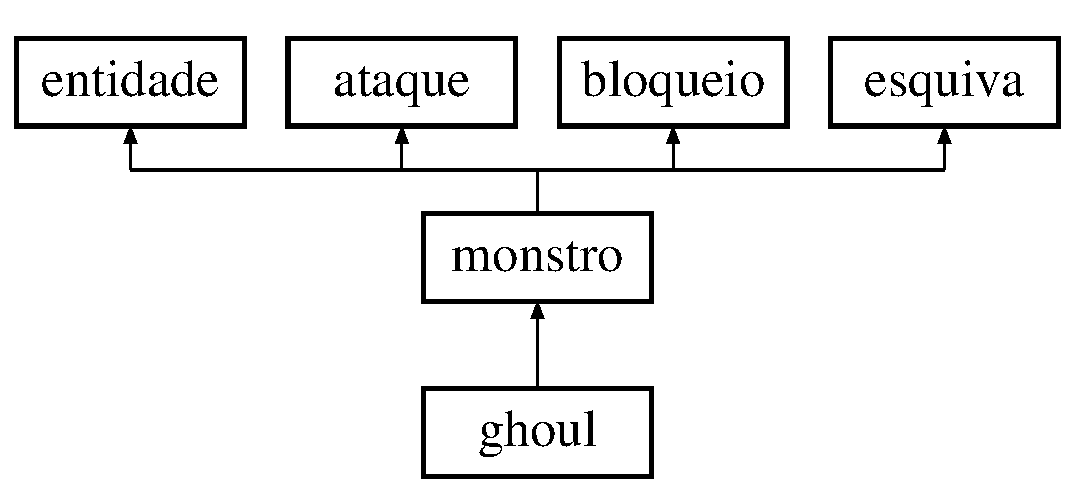
\includegraphics[height=3.000000cm]{classghoul}
\end{center}
\end{figure}
\subsection*{Public Member Functions}
\begin{DoxyCompactItemize}
\item 
\mbox{\hyperlink{classghoul_a35e44ea504998a44381e654defdd1202}{ghoul}} ()
\begin{DoxyCompactList}\small\item\em Criação classe ghoul. \end{DoxyCompactList}\end{DoxyCompactItemize}


\subsection{Constructor \& Destructor Documentation}
\mbox{\Hypertarget{classghoul_a35e44ea504998a44381e654defdd1202}\label{classghoul_a35e44ea504998a44381e654defdd1202}} 
\index{ghoul@{ghoul}!ghoul@{ghoul}}
\index{ghoul@{ghoul}!ghoul@{ghoul}}
\subsubsection{\texorpdfstring{ghoul()}{ghoul()}}
{\footnotesize\ttfamily ghoul\+::ghoul (\begin{DoxyParamCaption}{ }\end{DoxyParamCaption})}



Criação classe ghoul. 

Utilização da classe monstro como base. \begin{DoxyReturn}{Returns}
Objeto ghoul. 
\end{DoxyReturn}


The documentation for this class was generated from the following files\+:\begin{DoxyCompactItemize}
\item 
ghoul.\+h\item 
ghoul.\+cpp\end{DoxyCompactItemize}

\hypertarget{classmago}{}\section{mago Class Reference}
\label{classmago}\index{mago@{mago}}
Inheritance diagram for mago\+:\begin{figure}[H]
\begin{center}
\leavevmode
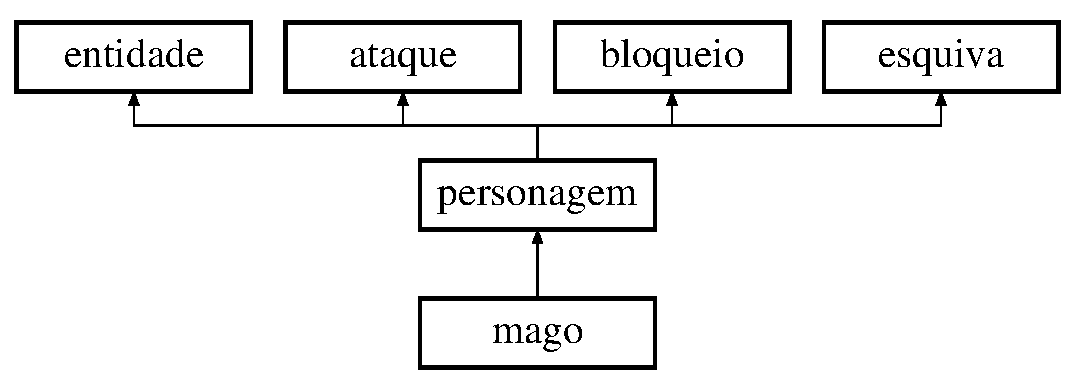
\includegraphics[height=3.000000cm]{classmago}
\end{center}
\end{figure}
\subsection*{Public Member Functions}
\begin{DoxyCompactItemize}
\item 
\mbox{\hyperlink{classmago_ae5292ae10f4e5cae0a4a73d185807fbc}{mago}} (string Nome)
\begin{DoxyCompactList}\small\item\em Criação da classe mago. \end{DoxyCompactList}\item 
int \mbox{\hyperlink{classmago_af10f6c9bcbbf77870f376a48b1cd0601}{controle\+Ataque}} (string valor, int arm\+Fisica, int arm\+Runica, int hp)
\begin{DoxyCompactList}\small\item\em Método de controle de ataque. \end{DoxyCompactList}\item 
int \mbox{\hyperlink{classmago_a039c9975fad5dbc54d5f3ab51bf3df44}{skill\+Um}} (int arm\+Fisica, int arm\+Runica, int hp)
\begin{DoxyCompactList}\small\item\em Método skill\+Um. \end{DoxyCompactList}\item 
int \mbox{\hyperlink{classmago_ac0a8309b459ab7f27f356eff72817c2f}{skill\+Dois}} (int arm\+Fisica, int arm\+Runica, int hp)
\begin{DoxyCompactList}\small\item\em Método skill dois. \end{DoxyCompactList}\item 
int \mbox{\hyperlink{classmago_a77280ba40aac7fdf8766950261821a39}{skill\+Tres}} (int arm\+Fisica, int arm\+Runica, int hp)
\begin{DoxyCompactList}\small\item\em Método skill três. \end{DoxyCompactList}\item 
void \mbox{\hyperlink{classmago_a8953a4898dea53c2c4a63542f49a7d86}{help}} ()
\begin{DoxyCompactList}\small\item\em Método help. \end{DoxyCompactList}\end{DoxyCompactItemize}


\subsection{Constructor \& Destructor Documentation}
\mbox{\Hypertarget{classmago_ae5292ae10f4e5cae0a4a73d185807fbc}\label{classmago_ae5292ae10f4e5cae0a4a73d185807fbc}} 
\index{mago@{mago}!mago@{mago}}
\index{mago@{mago}!mago@{mago}}
\subsubsection{\texorpdfstring{mago()}{mago()}}
{\footnotesize\ttfamily mago\+::mago (\begin{DoxyParamCaption}\item[{string}]{Nome }\end{DoxyParamCaption})}



Criação da classe mago. 

Utilização da classe personagem como base. \begin{DoxyReturn}{Returns}
Objeto mago. 
\end{DoxyReturn}


\subsection{Member Function Documentation}
\mbox{\Hypertarget{classmago_af10f6c9bcbbf77870f376a48b1cd0601}\label{classmago_af10f6c9bcbbf77870f376a48b1cd0601}} 
\index{mago@{mago}!controle\+Ataque@{controle\+Ataque}}
\index{controle\+Ataque@{controle\+Ataque}!mago@{mago}}
\subsubsection{\texorpdfstring{controle\+Ataque()}{controleAtaque()}}
{\footnotesize\ttfamily int mago\+::controle\+Ataque (\begin{DoxyParamCaption}\item[{string}]{valor,  }\item[{int}]{arm\+Fisica,  }\item[{int}]{arm\+Runica,  }\item[{int}]{hp }\end{DoxyParamCaption})}



Método de controle de ataque. 

recebe valor do usuário, armadura física, armadura mágica e hp do alvo. \begin{DoxyReturn}{Returns}
dano causado. 
\end{DoxyReturn}
\mbox{\Hypertarget{classmago_a8953a4898dea53c2c4a63542f49a7d86}\label{classmago_a8953a4898dea53c2c4a63542f49a7d86}} 
\index{mago@{mago}!help@{help}}
\index{help@{help}!mago@{mago}}
\subsubsection{\texorpdfstring{help()}{help()}}
{\footnotesize\ttfamily void mago\+::help (\begin{DoxyParamCaption}{ }\end{DoxyParamCaption})}



Método help. 

Informa ao jogador detalhes das skills. \begin{DoxyReturn}{Returns}
void. 
\end{DoxyReturn}
\mbox{\Hypertarget{classmago_ac0a8309b459ab7f27f356eff72817c2f}\label{classmago_ac0a8309b459ab7f27f356eff72817c2f}} 
\index{mago@{mago}!skill\+Dois@{skill\+Dois}}
\index{skill\+Dois@{skill\+Dois}!mago@{mago}}
\subsubsection{\texorpdfstring{skill\+Dois()}{skillDois()}}
{\footnotesize\ttfamily int mago\+::skill\+Dois (\begin{DoxyParamCaption}\item[{int}]{arm\+Fisica,  }\item[{int}]{arm\+Runica,  }\item[{int}]{hp }\end{DoxyParamCaption})}



Método skill dois. 

Skill de dano massivo baseado na mana, armadura rúnica e valor constante. \begin{DoxyReturn}{Returns}
Dano causado. 
\end{DoxyReturn}
\mbox{\Hypertarget{classmago_a77280ba40aac7fdf8766950261821a39}\label{classmago_a77280ba40aac7fdf8766950261821a39}} 
\index{mago@{mago}!skill\+Tres@{skill\+Tres}}
\index{skill\+Tres@{skill\+Tres}!mago@{mago}}
\subsubsection{\texorpdfstring{skill\+Tres()}{skillTres()}}
{\footnotesize\ttfamily int mago\+::skill\+Tres (\begin{DoxyParamCaption}\item[{int}]{arm\+Fisica,  }\item[{int}]{arm\+Runica,  }\item[{int}]{hp }\end{DoxyParamCaption})}



Método skill três. 

skill que aumenta o hp baseado na sua mana atual. \begin{DoxyReturn}{Returns}
Status melhorado. 
\end{DoxyReturn}
\mbox{\Hypertarget{classmago_a039c9975fad5dbc54d5f3ab51bf3df44}\label{classmago_a039c9975fad5dbc54d5f3ab51bf3df44}} 
\index{mago@{mago}!skill\+Um@{skill\+Um}}
\index{skill\+Um@{skill\+Um}!mago@{mago}}
\subsubsection{\texorpdfstring{skill\+Um()}{skillUm()}}
{\footnotesize\ttfamily int mago\+::skill\+Um (\begin{DoxyParamCaption}\item[{int}]{arm\+Fisica,  }\item[{int}]{arm\+Runica,  }\item[{int}]{hp }\end{DoxyParamCaption})}



Método skill\+Um. 

Aplica um dano baseado na armadura mágica, custa 30 de mana, ou dispara golpe simples. \begin{DoxyReturn}{Returns}
Dano causado. 
\end{DoxyReturn}


The documentation for this class was generated from the following files\+:\begin{DoxyCompactItemize}
\item 
mago.\+h\item 
mago.\+cpp\end{DoxyCompactItemize}

\hypertarget{classminotauro}{}\section{minotauro Class Reference}
\label{classminotauro}\index{minotauro@{minotauro}}
Inheritance diagram for minotauro\+:\begin{figure}[H]
\begin{center}
\leavevmode
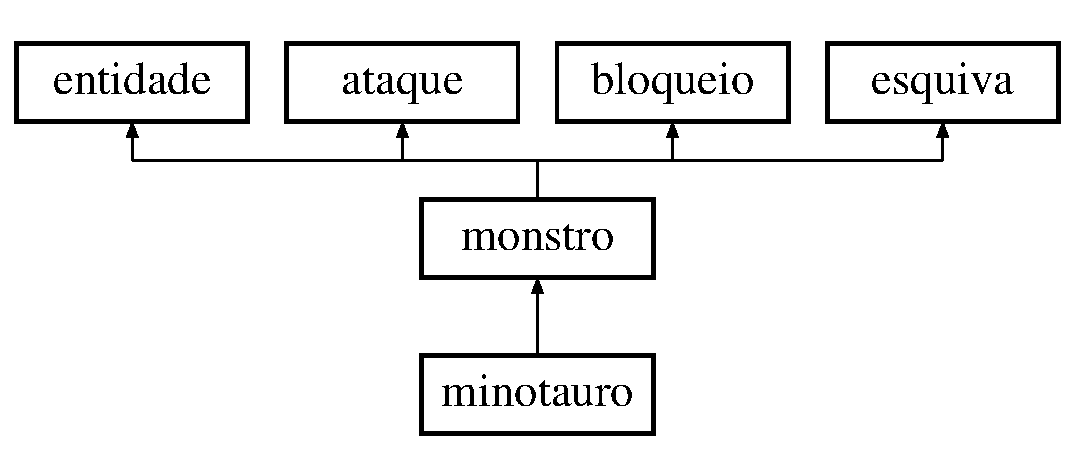
\includegraphics[height=3.000000cm]{classminotauro}
\end{center}
\end{figure}
\subsection*{Public Member Functions}
\begin{DoxyCompactItemize}
\item 
\mbox{\hyperlink{classminotauro_ae0c61c79540cae3c5afded22d870a449}{minotauro}} ()
\begin{DoxyCompactList}\small\item\em Criação da classe minotauro. \end{DoxyCompactList}\end{DoxyCompactItemize}


\subsection{Constructor \& Destructor Documentation}
\mbox{\Hypertarget{classminotauro_ae0c61c79540cae3c5afded22d870a449}\label{classminotauro_ae0c61c79540cae3c5afded22d870a449}} 
\index{minotauro@{minotauro}!minotauro@{minotauro}}
\index{minotauro@{minotauro}!minotauro@{minotauro}}
\subsubsection{\texorpdfstring{minotauro()}{minotauro()}}
{\footnotesize\ttfamily minotauro\+::minotauro (\begin{DoxyParamCaption}{ }\end{DoxyParamCaption})}



Criação da classe minotauro. 

Utilização da classe monstro como base. \begin{DoxyReturn}{Returns}
Objeto minotauro. 
\end{DoxyReturn}


The documentation for this class was generated from the following files\+:\begin{DoxyCompactItemize}
\item 
minotauro.\+h\item 
minotauro.\+cpp\end{DoxyCompactItemize}

\hypertarget{classmonstro}{}\section{monstro Class Reference}
\label{classmonstro}\index{monstro@{monstro}}
Inheritance diagram for monstro\+:\begin{figure}[H]
\begin{center}
\leavevmode
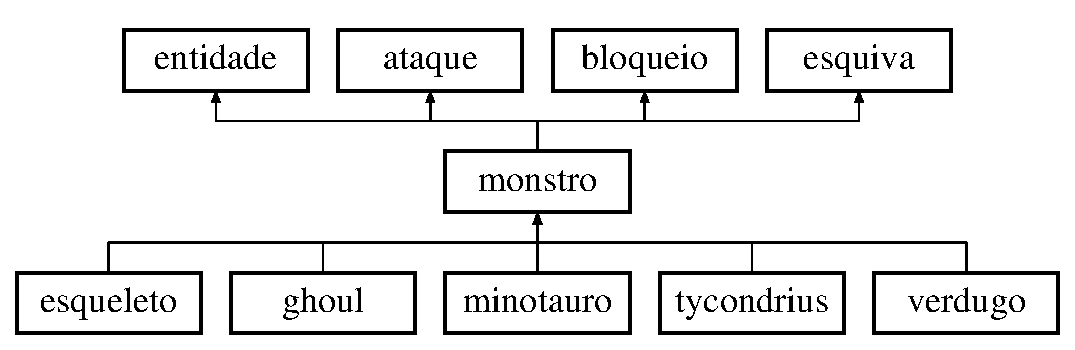
\includegraphics[height=3.000000cm]{classmonstro}
\end{center}
\end{figure}
\subsection*{Public Member Functions}
\begin{DoxyCompactItemize}
\item 
\mbox{\hyperlink{classmonstro_a0c7be686f5717cb625a3dabb75f6143f}{monstro}} (int valor\+Ataque, int hp, int mana, int arm\+Fisica, int arm\+Runica, int per\+Esquiva, string Nome, int Tipo)
\begin{DoxyCompactList}\small\item\em Criação da classe monstro. \end{DoxyCompactList}\item 
int \mbox{\hyperlink{classmonstro_a37425b0ce131bea83207142ef6b6c3bd}{realizar\+Ataque}} (int arm\+Fisica, int arm\+Runica, int hp)
\begin{DoxyCompactList}\small\item\em Método de controle de ataque. \end{DoxyCompactList}\item 
string \mbox{\hyperlink{classmonstro_a5b70fbe99ed64823246664deec8d4d6c}{get\+Nome}} ()
\begin{DoxyCompactList}\small\item\em Método get do nome. \end{DoxyCompactList}\item 
\mbox{\Hypertarget{classmonstro_a4855556c86824869d11cc9f4bda17beb}\label{classmonstro_a4855556c86824869d11cc9f4bda17beb}} 
int {\bfseries get\+Ataque} ()
\item 
int \mbox{\hyperlink{classmonstro_a5fbec06d53697ed81f0ca64136f7eb85}{get\+Hp}} ()
\begin{DoxyCompactList}\small\item\em Método get de HP. \end{DoxyCompactList}\item 
int \mbox{\hyperlink{classmonstro_abf4c7159c0370eef7ee5c1992f475746}{get\+M\+Ana}} ()
\begin{DoxyCompactList}\small\item\em Método get de mana. \end{DoxyCompactList}\item 
void \mbox{\hyperlink{classmonstro_a2753a130e042a12b9a5be36cb01deba5}{debitar\+Hp}} (int valor)
\begin{DoxyCompactList}\small\item\em Método de debitar HP do monstro. \end{DoxyCompactList}\item 
void \mbox{\hyperlink{classmonstro_a1dfc486d9da7e45f0afc2da3aebfe4f8}{debitar\+M\+Ana}} (int valor)
\begin{DoxyCompactList}\small\item\em Método de debitar mana do monstro. \end{DoxyCompactList}\item 
int \mbox{\hyperlink{classmonstro_ab7a3d4c7f9ca3e5f56e27c5a1716d70f}{get\+Sorteio}} ()
\begin{DoxyCompactList}\small\item\em Método de sorteia um dado D20. \end{DoxyCompactList}\item 
int \mbox{\hyperlink{classmonstro_ad13bd91217c356e1e4ef3e50ee4160aa}{Dano}} (int arm\+Fisica)
\begin{DoxyCompactList}\small\item\em Método de causar dano do monstro. \end{DoxyCompactList}\item 
int \mbox{\hyperlink{classmonstro_adc603e8df99ff928bdb1ffc1a95f604f}{get\+Arm\+Fisica}} ()
\begin{DoxyCompactList}\small\item\em Método get de armadura física. \end{DoxyCompactList}\item 
int \mbox{\hyperlink{classmonstro_abc73db4e55eb8c72aa433d4da43bd997}{get\+Arm\+Runica}} ()
\begin{DoxyCompactList}\small\item\em Método get de armadura runica. \end{DoxyCompactList}\item 
void \mbox{\hyperlink{classmonstro_a5935667552ab7ec9ccd94e4632ecb428}{set\+Arm\+Fisica}} (int valor)
\begin{DoxyCompactList}\small\item\em Método set de valor de armadura física. \end{DoxyCompactList}\item 
void \mbox{\hyperlink{classmonstro_a81c11a61a2dc1dc6536b3c3a75947060}{set\+Arm\+Runica}} (int valor)
\begin{DoxyCompactList}\small\item\em Método set de armadura runica. \end{DoxyCompactList}\item 
bool \mbox{\hyperlink{classmonstro_a256135af5123c6927214fd6ed6d72270}{Esquivar}} ()
\begin{DoxyCompactList}\small\item\em Método de esquivar do monstro. \end{DoxyCompactList}\end{DoxyCompactItemize}


\subsection{Constructor \& Destructor Documentation}
\mbox{\Hypertarget{classmonstro_a0c7be686f5717cb625a3dabb75f6143f}\label{classmonstro_a0c7be686f5717cb625a3dabb75f6143f}} 
\index{monstro@{monstro}!monstro@{monstro}}
\index{monstro@{monstro}!monstro@{monstro}}
\subsubsection{\texorpdfstring{monstro()}{monstro()}}
{\footnotesize\ttfamily monstro\+::monstro (\begin{DoxyParamCaption}\item[{int}]{valor\+Ataque,  }\item[{int}]{hp,  }\item[{int}]{mana,  }\item[{int}]{arm\+Fisica,  }\item[{int}]{arm\+Runica,  }\item[{int}]{per\+Esquiva,  }\item[{string}]{Nome,  }\item[{int}]{Tipo }\end{DoxyParamCaption})}



Criação da classe monstro. 

Utilização das classes ataque,bloqueio,entidade e esquiva como base. \begin{DoxyReturn}{Returns}
Objeto monstro. 
\end{DoxyReturn}


\subsection{Member Function Documentation}
\mbox{\Hypertarget{classmonstro_ad13bd91217c356e1e4ef3e50ee4160aa}\label{classmonstro_ad13bd91217c356e1e4ef3e50ee4160aa}} 
\index{monstro@{monstro}!Dano@{Dano}}
\index{Dano@{Dano}!monstro@{monstro}}
\subsubsection{\texorpdfstring{Dano()}{Dano()}}
{\footnotesize\ttfamily int monstro\+::\+Dano (\begin{DoxyParamCaption}\item[{int}]{arm\+Fisica }\end{DoxyParamCaption})}



Método de causar dano do monstro. 

se baseia no valor informado para aplicar dano com base na classe ataque. \begin{DoxyReturn}{Returns}
valor do dano a ser causado. 
\end{DoxyReturn}
\mbox{\Hypertarget{classmonstro_a2753a130e042a12b9a5be36cb01deba5}\label{classmonstro_a2753a130e042a12b9a5be36cb01deba5}} 
\index{monstro@{monstro}!debitar\+Hp@{debitar\+Hp}}
\index{debitar\+Hp@{debitar\+Hp}!monstro@{monstro}}
\subsubsection{\texorpdfstring{debitar\+Hp()}{debitarHp()}}
{\footnotesize\ttfamily void monstro\+::debitar\+Hp (\begin{DoxyParamCaption}\item[{int}]{valor }\end{DoxyParamCaption})}



Método de debitar HP do monstro. 

faz a redução do hp baseado no valor informado. \begin{DoxyReturn}{Returns}
void. 
\end{DoxyReturn}
\mbox{\Hypertarget{classmonstro_a1dfc486d9da7e45f0afc2da3aebfe4f8}\label{classmonstro_a1dfc486d9da7e45f0afc2da3aebfe4f8}} 
\index{monstro@{monstro}!debitar\+M\+Ana@{debitar\+M\+Ana}}
\index{debitar\+M\+Ana@{debitar\+M\+Ana}!monstro@{monstro}}
\subsubsection{\texorpdfstring{debitar\+M\+Ana()}{debitarMAna()}}
{\footnotesize\ttfamily void monstro\+::debitar\+M\+Ana (\begin{DoxyParamCaption}\item[{int}]{valor }\end{DoxyParamCaption})}



Método de debitar mana do monstro. 

faz a redução do mana baseado no valor informado. \begin{DoxyReturn}{Returns}
void. 
\end{DoxyReturn}
\mbox{\Hypertarget{classmonstro_a256135af5123c6927214fd6ed6d72270}\label{classmonstro_a256135af5123c6927214fd6ed6d72270}} 
\index{monstro@{monstro}!Esquivar@{Esquivar}}
\index{Esquivar@{Esquivar}!monstro@{monstro}}
\subsubsection{\texorpdfstring{Esquivar()}{Esquivar()}}
{\footnotesize\ttfamily bool monstro\+::\+Esquivar (\begin{DoxyParamCaption}{ }\end{DoxyParamCaption})}



Método de esquivar do monstro. 

Calcula a chance do usuário se esquivar de determinado dano. \begin{DoxyReturn}{Returns}
bool valor. 
\end{DoxyReturn}
\mbox{\Hypertarget{classmonstro_adc603e8df99ff928bdb1ffc1a95f604f}\label{classmonstro_adc603e8df99ff928bdb1ffc1a95f604f}} 
\index{monstro@{monstro}!get\+Arm\+Fisica@{get\+Arm\+Fisica}}
\index{get\+Arm\+Fisica@{get\+Arm\+Fisica}!monstro@{monstro}}
\subsubsection{\texorpdfstring{get\+Arm\+Fisica()}{getArmFisica()}}
{\footnotesize\ttfamily int monstro\+::get\+Arm\+Fisica (\begin{DoxyParamCaption}{ }\end{DoxyParamCaption})}



Método get de armadura física. 

\begin{DoxyReturn}{Returns}
armadura física do monstro. 
\end{DoxyReturn}
\mbox{\Hypertarget{classmonstro_abc73db4e55eb8c72aa433d4da43bd997}\label{classmonstro_abc73db4e55eb8c72aa433d4da43bd997}} 
\index{monstro@{monstro}!get\+Arm\+Runica@{get\+Arm\+Runica}}
\index{get\+Arm\+Runica@{get\+Arm\+Runica}!monstro@{monstro}}
\subsubsection{\texorpdfstring{get\+Arm\+Runica()}{getArmRunica()}}
{\footnotesize\ttfamily int monstro\+::get\+Arm\+Runica (\begin{DoxyParamCaption}{ }\end{DoxyParamCaption})}



Método get de armadura runica. 

\begin{DoxyReturn}{Returns}
armadura runica do monstro. 
\end{DoxyReturn}
\mbox{\Hypertarget{classmonstro_a5fbec06d53697ed81f0ca64136f7eb85}\label{classmonstro_a5fbec06d53697ed81f0ca64136f7eb85}} 
\index{monstro@{monstro}!get\+Hp@{get\+Hp}}
\index{get\+Hp@{get\+Hp}!monstro@{monstro}}
\subsubsection{\texorpdfstring{get\+Hp()}{getHp()}}
{\footnotesize\ttfamily int monstro\+::get\+Hp (\begin{DoxyParamCaption}{ }\end{DoxyParamCaption})}



Método get de HP. 

\begin{DoxyReturn}{Returns}
hp do monstro. 
\end{DoxyReturn}
\mbox{\Hypertarget{classmonstro_abf4c7159c0370eef7ee5c1992f475746}\label{classmonstro_abf4c7159c0370eef7ee5c1992f475746}} 
\index{monstro@{monstro}!get\+M\+Ana@{get\+M\+Ana}}
\index{get\+M\+Ana@{get\+M\+Ana}!monstro@{monstro}}
\subsubsection{\texorpdfstring{get\+M\+Ana()}{getMAna()}}
{\footnotesize\ttfamily int monstro\+::get\+M\+Ana (\begin{DoxyParamCaption}{ }\end{DoxyParamCaption})}



Método get de mana. 

\begin{DoxyReturn}{Returns}
mana do monstro. 
\end{DoxyReturn}
\mbox{\Hypertarget{classmonstro_a5b70fbe99ed64823246664deec8d4d6c}\label{classmonstro_a5b70fbe99ed64823246664deec8d4d6c}} 
\index{monstro@{monstro}!get\+Nome@{get\+Nome}}
\index{get\+Nome@{get\+Nome}!monstro@{monstro}}
\subsubsection{\texorpdfstring{get\+Nome()}{getNome()}}
{\footnotesize\ttfamily string monstro\+::get\+Nome (\begin{DoxyParamCaption}{ }\end{DoxyParamCaption})}



Método get do nome. 

\begin{DoxyReturn}{Returns}
nome do monstro. 
\end{DoxyReturn}
\mbox{\Hypertarget{classmonstro_ab7a3d4c7f9ca3e5f56e27c5a1716d70f}\label{classmonstro_ab7a3d4c7f9ca3e5f56e27c5a1716d70f}} 
\index{monstro@{monstro}!get\+Sorteio@{get\+Sorteio}}
\index{get\+Sorteio@{get\+Sorteio}!monstro@{monstro}}
\subsubsection{\texorpdfstring{get\+Sorteio()}{getSorteio()}}
{\footnotesize\ttfamily int monstro\+::get\+Sorteio (\begin{DoxyParamCaption}{ }\end{DoxyParamCaption})}



Método de sorteia um dado D20. 

faz o sorteio do valor para o método controle de ataque. \begin{DoxyReturn}{Returns}
valor de 1 a 20. 
\end{DoxyReturn}
\mbox{\Hypertarget{classmonstro_a37425b0ce131bea83207142ef6b6c3bd}\label{classmonstro_a37425b0ce131bea83207142ef6b6c3bd}} 
\index{monstro@{monstro}!realizar\+Ataque@{realizar\+Ataque}}
\index{realizar\+Ataque@{realizar\+Ataque}!monstro@{monstro}}
\subsubsection{\texorpdfstring{realizar\+Ataque()}{realizarAtaque()}}
{\footnotesize\ttfamily int monstro\+::realizar\+Ataque (\begin{DoxyParamCaption}\item[{int}]{arm\+Fisica,  }\item[{int}]{arm\+Runica,  }\item[{int}]{hp }\end{DoxyParamCaption})}



Método de controle de ataque. 

recebe valor do usuário, armadura física, armadura mágica e hp do alvo. \begin{DoxyReturn}{Returns}
dano causado. 
\end{DoxyReturn}
\mbox{\Hypertarget{classmonstro_a5935667552ab7ec9ccd94e4632ecb428}\label{classmonstro_a5935667552ab7ec9ccd94e4632ecb428}} 
\index{monstro@{monstro}!set\+Arm\+Fisica@{set\+Arm\+Fisica}}
\index{set\+Arm\+Fisica@{set\+Arm\+Fisica}!monstro@{monstro}}
\subsubsection{\texorpdfstring{set\+Arm\+Fisica()}{setArmFisica()}}
{\footnotesize\ttfamily void monstro\+::set\+Arm\+Fisica (\begin{DoxyParamCaption}\item[{int}]{valor }\end{DoxyParamCaption})}



Método set de valor de armadura física. 

\begin{DoxyReturn}{Returns}

\end{DoxyReturn}
\mbox{\Hypertarget{classmonstro_a81c11a61a2dc1dc6536b3c3a75947060}\label{classmonstro_a81c11a61a2dc1dc6536b3c3a75947060}} 
\index{monstro@{monstro}!set\+Arm\+Runica@{set\+Arm\+Runica}}
\index{set\+Arm\+Runica@{set\+Arm\+Runica}!monstro@{monstro}}
\subsubsection{\texorpdfstring{set\+Arm\+Runica()}{setArmRunica()}}
{\footnotesize\ttfamily void monstro\+::set\+Arm\+Runica (\begin{DoxyParamCaption}\item[{int}]{valor }\end{DoxyParamCaption})}



Método set de armadura runica. 

\begin{DoxyReturn}{Returns}

\end{DoxyReturn}


The documentation for this class was generated from the following files\+:\begin{DoxyCompactItemize}
\item 
monstros.\+h\item 
monstros.\+cpp\end{DoxyCompactItemize}

\hypertarget{classpaladino}{}\section{paladino Class Reference}
\label{classpaladino}\index{paladino@{paladino}}
Inheritance diagram for paladino\+:\begin{figure}[H]
\begin{center}
\leavevmode
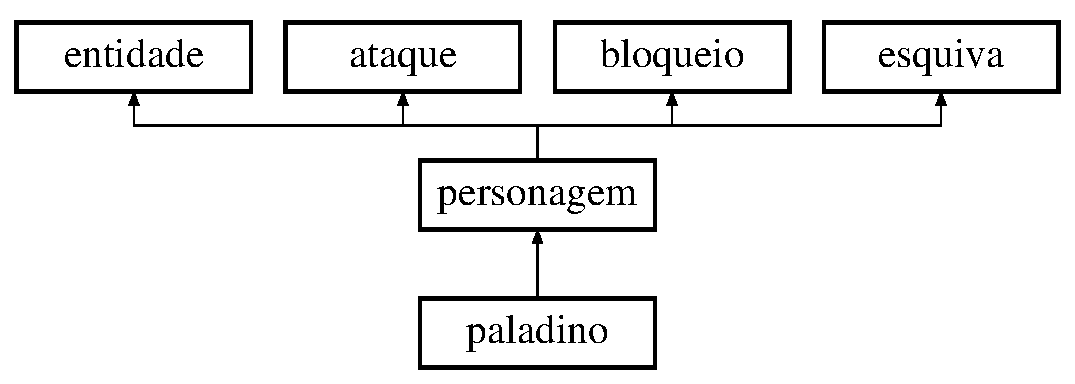
\includegraphics[height=3.000000cm]{classpaladino}
\end{center}
\end{figure}
\subsection*{Public Member Functions}
\begin{DoxyCompactItemize}
\item 
\mbox{\hyperlink{classpaladino_a312e5f9a43967aa31e34128051646277}{paladino}} (string Nome)
\begin{DoxyCompactList}\small\item\em Criação da classe paladino. \end{DoxyCompactList}\item 
int \mbox{\hyperlink{classpaladino_a059fd05922c2adcbd87743b9c3552c11}{controle\+Ataque}} (string valor, int arm\+Fisica, int arm\+Runica, int hp)
\begin{DoxyCompactList}\small\item\em Método de controle de ataque. \end{DoxyCompactList}\item 
int \mbox{\hyperlink{classpaladino_aaf70250e226146bab3bb421b253483d5}{skill\+Um}} (int arm\+Fisica, int arm\+Runica, int hp)
\begin{DoxyCompactList}\small\item\em Método skill\+Um. \end{DoxyCompactList}\item 
int \mbox{\hyperlink{classpaladino_a62a3129268222902926377c6dd0dceb5}{skill\+Dois}} (int arm\+Fisica, int arm\+Runica, int hp)
\begin{DoxyCompactList}\small\item\em Método skill dois. \end{DoxyCompactList}\item 
int \mbox{\hyperlink{classpaladino_acd4e68058d2504c07989af88ace6d57b}{skill\+Tres}} (int arm\+Fisica, int arm\+Runica, int hp)
<<<<<<< HEAD
\begin{DoxyCompactList}\small\item\em Método skill\+Tres. \end{DoxyCompactList}\item 
void \mbox{\hyperlink{classpaladino_a028019d72c919de0589cccdfed402a18}{help}} ()
\begin{DoxyCompactList}\small\item\em Método help. \end{DoxyCompactList}\end{DoxyCompactItemize}
=======
\begin{DoxyCompactList}\small\item\em Método skill\+Tres. \end{DoxyCompactList}\end{DoxyCompactItemize}
>>>>>>> 0546f94c50e08ebf892bc8350edb40cb6ecd7634


\subsection{Constructor \& Destructor Documentation}
\mbox{\Hypertarget{classpaladino_a312e5f9a43967aa31e34128051646277}\label{classpaladino_a312e5f9a43967aa31e34128051646277}} 
\index{paladino@{paladino}!paladino@{paladino}}
\index{paladino@{paladino}!paladino@{paladino}}
\subsubsection{\texorpdfstring{paladino()}{paladino()}}
{\footnotesize\ttfamily paladino\+::paladino (\begin{DoxyParamCaption}\item[{string}]{Nome }\end{DoxyParamCaption})}



Criação da classe paladino. 

Utilização da classe personagem como base. \begin{DoxyReturn}{Returns}
Objeto paladino. 
\end{DoxyReturn}


\subsection{Member Function Documentation}
\mbox{\Hypertarget{classpaladino_a059fd05922c2adcbd87743b9c3552c11}\label{classpaladino_a059fd05922c2adcbd87743b9c3552c11}} 
\index{paladino@{paladino}!controle\+Ataque@{controle\+Ataque}}
\index{controle\+Ataque@{controle\+Ataque}!paladino@{paladino}}
\subsubsection{\texorpdfstring{controle\+Ataque()}{controleAtaque()}}
{\footnotesize\ttfamily int paladino\+::controle\+Ataque (\begin{DoxyParamCaption}\item[{string}]{valor,  }\item[{int}]{arm\+Fisica,  }\item[{int}]{arm\+Runica,  }\item[{int}]{hp }\end{DoxyParamCaption})}



Método de controle de ataque. 

recebe valor do usuário, armadura física, armadura mágica e hp do alvo. \begin{DoxyReturn}{Returns}
dano causado. 
\end{DoxyReturn}
<<<<<<< HEAD
\mbox{\Hypertarget{classpaladino_a028019d72c919de0589cccdfed402a18}\label{classpaladino_a028019d72c919de0589cccdfed402a18}} 
\index{paladino@{paladino}!help@{help}}
\index{help@{help}!paladino@{paladino}}
\subsubsection{\texorpdfstring{help()}{help()}}
{\footnotesize\ttfamily void paladino\+::help (\begin{DoxyParamCaption}{ }\end{DoxyParamCaption})}



Método help. 

Informa ao jogador detalhes das skills. \begin{DoxyReturn}{Returns}
void. 
\end{DoxyReturn}
=======
>>>>>>> 0546f94c50e08ebf892bc8350edb40cb6ecd7634
\mbox{\Hypertarget{classpaladino_a62a3129268222902926377c6dd0dceb5}\label{classpaladino_a62a3129268222902926377c6dd0dceb5}} 
\index{paladino@{paladino}!skill\+Dois@{skill\+Dois}}
\index{skill\+Dois@{skill\+Dois}!paladino@{paladino}}
\subsubsection{\texorpdfstring{skill\+Dois()}{skillDois()}}
{\footnotesize\ttfamily int paladino\+::skill\+Dois (\begin{DoxyParamCaption}\item[{int}]{arm\+Fisica,  }\item[{int}]{arm\+Runica,  }\item[{int}]{hp }\end{DoxyParamCaption})}



Método skill dois. 

Dano simples baseado na armadura física, custa 10 de mana. \begin{DoxyReturn}{Returns}
Dano causado. 
\end{DoxyReturn}
\mbox{\Hypertarget{classpaladino_acd4e68058d2504c07989af88ace6d57b}\label{classpaladino_acd4e68058d2504c07989af88ace6d57b}} 
\index{paladino@{paladino}!skill\+Tres@{skill\+Tres}}
\index{skill\+Tres@{skill\+Tres}!paladino@{paladino}}
\subsubsection{\texorpdfstring{skill\+Tres()}{skillTres()}}
{\footnotesize\ttfamily int paladino\+::skill\+Tres (\begin{DoxyParamCaption}\item[{int}]{arm\+Fisica,  }\item[{int}]{arm\+Runica,  }\item[{int}]{hp }\end{DoxyParamCaption})}



Método skill\+Tres. 

Aumenta o dano da arma em +10,custa 10 de mana. \begin{DoxyReturn}{Returns}
Status melhorado. 
\end{DoxyReturn}
\mbox{\Hypertarget{classpaladino_aaf70250e226146bab3bb421b253483d5}\label{classpaladino_aaf70250e226146bab3bb421b253483d5}} 
\index{paladino@{paladino}!skill\+Um@{skill\+Um}}
\index{skill\+Um@{skill\+Um}!paladino@{paladino}}
\subsubsection{\texorpdfstring{skill\+Um()}{skillUm()}}
{\footnotesize\ttfamily int paladino\+::skill\+Um (\begin{DoxyParamCaption}\item[{int}]{arm\+Fisica,  }\item[{int}]{arm\+Runica,  }\item[{int}]{hp }\end{DoxyParamCaption})}



Método skill\+Um. 

Dano baseado na armadura física e mágica do alvo a custo de 30 de mana. \begin{DoxyReturn}{Returns}
Dano causado. 
\end{DoxyReturn}


The documentation for this class was generated from the following files\+:\begin{DoxyCompactItemize}
\item 
paladino.\+h\item 
paladino.\+cpp\end{DoxyCompactItemize}

\hypertarget{classpersonagem}{}\section{personagem Class Reference}
\label{classpersonagem}\index{personagem@{personagem}}
Inheritance diagram for personagem\+:\begin{figure}[H]
\begin{center}
\leavevmode
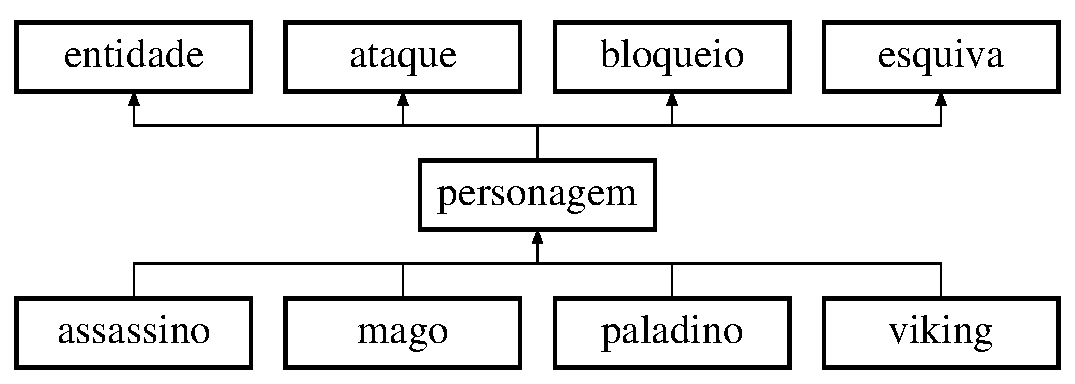
\includegraphics[height=3.000000cm]{classpersonagem}
\end{center}
\end{figure}
\subsection*{Public Member Functions}
\begin{DoxyCompactItemize}
\item 
\mbox{\hyperlink{classpersonagem_ab07283c6d509230657835ef6ceed411d}{personagem}} (int valor\+Ataque, int hp, int mana, int arm\+Fisica, int arm\+Runica, int per\+Esquiva, string Nome)
\begin{DoxyCompactList}\small\item\em Criação da classe personagem. \end{DoxyCompactList}\item 
int \mbox{\hyperlink{classpersonagem_a6df830166e074493fe0a25502ec24d4d}{skill\+Um}} (int arm\+Fisica, int arm\+Runica, int hp)
\begin{DoxyCompactList}\small\item\em Métodos de skills para serem sobescritos, da skill\+Um a skill\+Tres. \end{DoxyCompactList}\item 
\mbox{\Hypertarget{classpersonagem_aaa7cac0258a6e6e42c1b1d17ecbf3139}\label{classpersonagem_aaa7cac0258a6e6e42c1b1d17ecbf3139}} 
int {\bfseries skill\+Dois} (int arm\+Fisica, int arm\+Runica, int hp)
\item 
\mbox{\Hypertarget{classpersonagem_a015143bbe13eca5865f6e7eca45407cb}\label{classpersonagem_a015143bbe13eca5865f6e7eca45407cb}} 
int {\bfseries skill\+Tres} (int arm\+Fisica, int arm\+Runica, int hp)
\item 
int \mbox{\hyperlink{classpersonagem_a31e7891af5a68142e7dc693d894069f1}{controle\+Ataque}} (string valor, int arm\+Fisica, int arm\+Runica, int hp)
\begin{DoxyCompactList}\small\item\em Método de controle de ataque. \end{DoxyCompactList}\item 
string \mbox{\hyperlink{classpersonagem_a9b58d2e434e2fbc15786ce24bdf593ec}{get\+Nome}} ()
\begin{DoxyCompactList}\small\item\em Método get do nome. \end{DoxyCompactList}\item 
int \mbox{\hyperlink{classpersonagem_a70a912dec9dcdedffa208fb3a709fa57}{get\+Ataque}} ()
\begin{DoxyCompactList}\small\item\em Método get de ataque. \end{DoxyCompactList}\item 
void \mbox{\hyperlink{classpersonagem_a5f5f95e0fd8e5ceda996925c37cf6c4f}{set\+Ataq}} (int valor)
\begin{DoxyCompactList}\small\item\em Método set de valor de ataque. \end{DoxyCompactList}\item 
int \mbox{\hyperlink{classpersonagem_aae06914f2a7ab169b55863d5915341b3}{get\+Hp}} ()
\begin{DoxyCompactList}\small\item\em Método get de HP. \end{DoxyCompactList}\item 
int \mbox{\hyperlink{classpersonagem_acb34b3c679e4488e624ea53faf6aef62}{get\+M\+Ana}} ()
\begin{DoxyCompactList}\small\item\em Método get de mana. \end{DoxyCompactList}\item 
void \mbox{\hyperlink{classpersonagem_a71499a8c512467cf812e0bca2b3e2989}{debitar\+Hp}} (int valor)
\begin{DoxyCompactList}\small\item\em Método de debitar HP do personagem. \end{DoxyCompactList}\item 
void \mbox{\hyperlink{classpersonagem_a785a1a249510545caa1d08652351f22c}{debitar\+M\+Ana}} (int valor)
\begin{DoxyCompactList}\small\item\em Método de debitar mana do personagem. \end{DoxyCompactList}\item 
int \mbox{\hyperlink{classpersonagem_ae0c22f0be89d748e1b9c4752b704e80a}{Dano}} (int arm\+Fisica)
\begin{DoxyCompactList}\small\item\em Método de causar dano do personagem. \end{DoxyCompactList}\item 
int \mbox{\hyperlink{classpersonagem_a4a98195a030276936d22931f7ae9f37a}{get\+Arm\+Fisica}} ()
\begin{DoxyCompactList}\small\item\em Método get de armadura física. \end{DoxyCompactList}\item 
int \mbox{\hyperlink{classpersonagem_a1cbd2b54e1727407426a92bf2dcad39f}{get\+Arm\+Runica}} ()
\begin{DoxyCompactList}\small\item\em Método get de armadura runica. \end{DoxyCompactList}\item 
void \mbox{\hyperlink{classpersonagem_ac1561638f8684db27731b49ddbc5c386}{set\+Arm\+Fisica}} (int valor)
\begin{DoxyCompactList}\small\item\em Método set de valor de armadura física. \end{DoxyCompactList}\item 
void \mbox{\hyperlink{classpersonagem_aad825560abd7cd0a8760d4ee38baa612}{set\+Arm\+Runica}} (int valor)
\begin{DoxyCompactList}\small\item\em Método set de armadura runica. \end{DoxyCompactList}\item 
void \mbox{\hyperlink{classpersonagem_a9805607809f9b49ab19e3f02f20c86a2}{set\+Hp}} (int valor)
\begin{DoxyCompactList}\small\item\em Método set de HP do personagem. \end{DoxyCompactList}\item 
void \mbox{\hyperlink{classpersonagem_a40f2128ed721ed117a6e03c026082700}{set\+M\+Ana}} (int valor)
\begin{DoxyCompactList}\small\item\em Método set de mana do personagem. \end{DoxyCompactList}\item 
void \mbox{\hyperlink{classpersonagem_ab1c07cf6fcd0831d83ba624af01f9f04}{set\+Esquiv}} (int valor)
\begin{DoxyCompactList}\small\item\em Método set de esquiva do personagem. \end{DoxyCompactList}\item 
bool \mbox{\hyperlink{classpersonagem_ad03eea0bb9c6eec82fec3202da055309}{Esquivar}} ()
\begin{DoxyCompactList}\small\item\em Método de esquivar do personagem. \end{DoxyCompactList}\end{DoxyCompactItemize}


\subsection{Constructor \& Destructor Documentation}
\mbox{\Hypertarget{classpersonagem_ab07283c6d509230657835ef6ceed411d}\label{classpersonagem_ab07283c6d509230657835ef6ceed411d}} 
\index{personagem@{personagem}!personagem@{personagem}}
\index{personagem@{personagem}!personagem@{personagem}}
\subsubsection{\texorpdfstring{personagem()}{personagem()}}
{\footnotesize\ttfamily personagem\+::personagem (\begin{DoxyParamCaption}\item[{int}]{valor\+Ataque,  }\item[{int}]{hp,  }\item[{int}]{mana,  }\item[{int}]{arm\+Fisica,  }\item[{int}]{arm\+Runica,  }\item[{int}]{per\+Esquiva,  }\item[{string}]{Nome }\end{DoxyParamCaption})}



Criação da classe personagem. 

Utilização das classes ataque,bloqueio,entidade e esquiva como base. \begin{DoxyReturn}{Returns}
Objeto personagem. 
\end{DoxyReturn}


\subsection{Member Function Documentation}
\mbox{\Hypertarget{classpersonagem_a31e7891af5a68142e7dc693d894069f1}\label{classpersonagem_a31e7891af5a68142e7dc693d894069f1}} 
\index{personagem@{personagem}!controle\+Ataque@{controle\+Ataque}}
\index{controle\+Ataque@{controle\+Ataque}!personagem@{personagem}}
\subsubsection{\texorpdfstring{controle\+Ataque()}{controleAtaque()}}
{\footnotesize\ttfamily int personagem\+::controle\+Ataque (\begin{DoxyParamCaption}\item[{string}]{valor,  }\item[{int}]{arm\+Fisica,  }\item[{int}]{arm\+Runica,  }\item[{int}]{hp }\end{DoxyParamCaption})}



Método de controle de ataque. 

recebe valor do usuário, armadura física, armadura mágica e hp do alvo. \begin{DoxyReturn}{Returns}
dano causado. 
\end{DoxyReturn}
\mbox{\Hypertarget{classpersonagem_ae0c22f0be89d748e1b9c4752b704e80a}\label{classpersonagem_ae0c22f0be89d748e1b9c4752b704e80a}} 
\index{personagem@{personagem}!Dano@{Dano}}
\index{Dano@{Dano}!personagem@{personagem}}
\subsubsection{\texorpdfstring{Dano()}{Dano()}}
{\footnotesize\ttfamily int personagem\+::\+Dano (\begin{DoxyParamCaption}\item[{int}]{arm\+Fisica }\end{DoxyParamCaption})}



Método de causar dano do personagem. 

se baseia no valor informado para aplicar dano com base na classe ataque. \begin{DoxyReturn}{Returns}
valor do dano a ser causado. 
\end{DoxyReturn}
\mbox{\Hypertarget{classpersonagem_a71499a8c512467cf812e0bca2b3e2989}\label{classpersonagem_a71499a8c512467cf812e0bca2b3e2989}} 
\index{personagem@{personagem}!debitar\+Hp@{debitar\+Hp}}
\index{debitar\+Hp@{debitar\+Hp}!personagem@{personagem}}
\subsubsection{\texorpdfstring{debitar\+Hp()}{debitarHp()}}
{\footnotesize\ttfamily void personagem\+::debitar\+Hp (\begin{DoxyParamCaption}\item[{int}]{valor }\end{DoxyParamCaption})}



Método de debitar HP do personagem. 

faz a redução do hp baseado no valor informado. \begin{DoxyReturn}{Returns}
void. 
\end{DoxyReturn}
\mbox{\Hypertarget{classpersonagem_a785a1a249510545caa1d08652351f22c}\label{classpersonagem_a785a1a249510545caa1d08652351f22c}} 
\index{personagem@{personagem}!debitar\+M\+Ana@{debitar\+M\+Ana}}
\index{debitar\+M\+Ana@{debitar\+M\+Ana}!personagem@{personagem}}
\subsubsection{\texorpdfstring{debitar\+M\+Ana()}{debitarMAna()}}
{\footnotesize\ttfamily void personagem\+::debitar\+M\+Ana (\begin{DoxyParamCaption}\item[{int}]{valor }\end{DoxyParamCaption})}



Método de debitar mana do personagem. 

faz a redução do mana baseado no valor informado. \begin{DoxyReturn}{Returns}
void. 
\end{DoxyReturn}
\mbox{\Hypertarget{classpersonagem_ad03eea0bb9c6eec82fec3202da055309}\label{classpersonagem_ad03eea0bb9c6eec82fec3202da055309}} 
\index{personagem@{personagem}!Esquivar@{Esquivar}}
\index{Esquivar@{Esquivar}!personagem@{personagem}}
\subsubsection{\texorpdfstring{Esquivar()}{Esquivar()}}
{\footnotesize\ttfamily bool personagem\+::\+Esquivar (\begin{DoxyParamCaption}{ }\end{DoxyParamCaption})}



Método de esquivar do personagem. 

Calcula a chance do usuário se esquivar de determinado dano. \begin{DoxyReturn}{Returns}
bool valor. 
\end{DoxyReturn}
\mbox{\Hypertarget{classpersonagem_a4a98195a030276936d22931f7ae9f37a}\label{classpersonagem_a4a98195a030276936d22931f7ae9f37a}} 
\index{personagem@{personagem}!get\+Arm\+Fisica@{get\+Arm\+Fisica}}
\index{get\+Arm\+Fisica@{get\+Arm\+Fisica}!personagem@{personagem}}
\subsubsection{\texorpdfstring{get\+Arm\+Fisica()}{getArmFisica()}}
{\footnotesize\ttfamily int personagem\+::get\+Arm\+Fisica (\begin{DoxyParamCaption}{ }\end{DoxyParamCaption})}



Método get de armadura física. 

\begin{DoxyReturn}{Returns}
armadura física do personagem. 
\end{DoxyReturn}
\mbox{\Hypertarget{classpersonagem_a1cbd2b54e1727407426a92bf2dcad39f}\label{classpersonagem_a1cbd2b54e1727407426a92bf2dcad39f}} 
\index{personagem@{personagem}!get\+Arm\+Runica@{get\+Arm\+Runica}}
\index{get\+Arm\+Runica@{get\+Arm\+Runica}!personagem@{personagem}}
\subsubsection{\texorpdfstring{get\+Arm\+Runica()}{getArmRunica()}}
{\footnotesize\ttfamily int personagem\+::get\+Arm\+Runica (\begin{DoxyParamCaption}{ }\end{DoxyParamCaption})}



Método get de armadura runica. 

\begin{DoxyReturn}{Returns}
armadura runica do personagem. 
\end{DoxyReturn}
\mbox{\Hypertarget{classpersonagem_a70a912dec9dcdedffa208fb3a709fa57}\label{classpersonagem_a70a912dec9dcdedffa208fb3a709fa57}} 
\index{personagem@{personagem}!get\+Ataque@{get\+Ataque}}
\index{get\+Ataque@{get\+Ataque}!personagem@{personagem}}
\subsubsection{\texorpdfstring{get\+Ataque()}{getAtaque()}}
{\footnotesize\ttfamily int personagem\+::get\+Ataque (\begin{DoxyParamCaption}{ }\end{DoxyParamCaption})}



Método get de ataque. 

\begin{DoxyReturn}{Returns}
ataque do personagem. 
\end{DoxyReturn}
\mbox{\Hypertarget{classpersonagem_aae06914f2a7ab169b55863d5915341b3}\label{classpersonagem_aae06914f2a7ab169b55863d5915341b3}} 
\index{personagem@{personagem}!get\+Hp@{get\+Hp}}
\index{get\+Hp@{get\+Hp}!personagem@{personagem}}
\subsubsection{\texorpdfstring{get\+Hp()}{getHp()}}
{\footnotesize\ttfamily int personagem\+::get\+Hp (\begin{DoxyParamCaption}{ }\end{DoxyParamCaption})}



Método get de HP. 

\begin{DoxyReturn}{Returns}
hp do personagem. 
\end{DoxyReturn}
\mbox{\Hypertarget{classpersonagem_acb34b3c679e4488e624ea53faf6aef62}\label{classpersonagem_acb34b3c679e4488e624ea53faf6aef62}} 
\index{personagem@{personagem}!get\+M\+Ana@{get\+M\+Ana}}
\index{get\+M\+Ana@{get\+M\+Ana}!personagem@{personagem}}
\subsubsection{\texorpdfstring{get\+M\+Ana()}{getMAna()}}
{\footnotesize\ttfamily int personagem\+::get\+M\+Ana (\begin{DoxyParamCaption}{ }\end{DoxyParamCaption})}



Método get de mana. 

\begin{DoxyReturn}{Returns}
mana do personagem. 
\end{DoxyReturn}
\mbox{\Hypertarget{classpersonagem_a9b58d2e434e2fbc15786ce24bdf593ec}\label{classpersonagem_a9b58d2e434e2fbc15786ce24bdf593ec}} 
\index{personagem@{personagem}!get\+Nome@{get\+Nome}}
\index{get\+Nome@{get\+Nome}!personagem@{personagem}}
\subsubsection{\texorpdfstring{get\+Nome()}{getNome()}}
{\footnotesize\ttfamily string personagem\+::get\+Nome (\begin{DoxyParamCaption}{ }\end{DoxyParamCaption})}



Método get do nome. 

\begin{DoxyReturn}{Returns}
nome do personagem. 
\end{DoxyReturn}
\mbox{\Hypertarget{classpersonagem_ac1561638f8684db27731b49ddbc5c386}\label{classpersonagem_ac1561638f8684db27731b49ddbc5c386}} 
\index{personagem@{personagem}!set\+Arm\+Fisica@{set\+Arm\+Fisica}}
\index{set\+Arm\+Fisica@{set\+Arm\+Fisica}!personagem@{personagem}}
\subsubsection{\texorpdfstring{set\+Arm\+Fisica()}{setArmFisica()}}
{\footnotesize\ttfamily void personagem\+::set\+Arm\+Fisica (\begin{DoxyParamCaption}\item[{int}]{valor }\end{DoxyParamCaption})}



Método set de valor de armadura física. 

\begin{DoxyReturn}{Returns}

\end{DoxyReturn}
\mbox{\Hypertarget{classpersonagem_aad825560abd7cd0a8760d4ee38baa612}\label{classpersonagem_aad825560abd7cd0a8760d4ee38baa612}} 
\index{personagem@{personagem}!set\+Arm\+Runica@{set\+Arm\+Runica}}
\index{set\+Arm\+Runica@{set\+Arm\+Runica}!personagem@{personagem}}
\subsubsection{\texorpdfstring{set\+Arm\+Runica()}{setArmRunica()}}
{\footnotesize\ttfamily void personagem\+::set\+Arm\+Runica (\begin{DoxyParamCaption}\item[{int}]{valor }\end{DoxyParamCaption})}



Método set de armadura runica. 

\begin{DoxyReturn}{Returns}

\end{DoxyReturn}
\mbox{\Hypertarget{classpersonagem_a5f5f95e0fd8e5ceda996925c37cf6c4f}\label{classpersonagem_a5f5f95e0fd8e5ceda996925c37cf6c4f}} 
\index{personagem@{personagem}!set\+Ataq@{set\+Ataq}}
\index{set\+Ataq@{set\+Ataq}!personagem@{personagem}}
\subsubsection{\texorpdfstring{set\+Ataq()}{setAtaq()}}
{\footnotesize\ttfamily void personagem\+::set\+Ataq (\begin{DoxyParamCaption}\item[{int}]{valor }\end{DoxyParamCaption})}



Método set de valor de ataque. 

\begin{DoxyReturn}{Returns}

\end{DoxyReturn}
\mbox{\Hypertarget{classpersonagem_ab1c07cf6fcd0831d83ba624af01f9f04}\label{classpersonagem_ab1c07cf6fcd0831d83ba624af01f9f04}} 
\index{personagem@{personagem}!set\+Esquiv@{set\+Esquiv}}
\index{set\+Esquiv@{set\+Esquiv}!personagem@{personagem}}
\subsubsection{\texorpdfstring{set\+Esquiv()}{setEsquiv()}}
{\footnotesize\ttfamily void personagem\+::set\+Esquiv (\begin{DoxyParamCaption}\item[{int}]{valor }\end{DoxyParamCaption})}



Método set de esquiva do personagem. 

\begin{DoxyReturn}{Returns}

\end{DoxyReturn}
\mbox{\Hypertarget{classpersonagem_a9805607809f9b49ab19e3f02f20c86a2}\label{classpersonagem_a9805607809f9b49ab19e3f02f20c86a2}} 
\index{personagem@{personagem}!set\+Hp@{set\+Hp}}
\index{set\+Hp@{set\+Hp}!personagem@{personagem}}
\subsubsection{\texorpdfstring{set\+Hp()}{setHp()}}
{\footnotesize\ttfamily void personagem\+::set\+Hp (\begin{DoxyParamCaption}\item[{int}]{valor }\end{DoxyParamCaption})}



Método set de HP do personagem. 

\begin{DoxyReturn}{Returns}

\end{DoxyReturn}
\mbox{\Hypertarget{classpersonagem_a40f2128ed721ed117a6e03c026082700}\label{classpersonagem_a40f2128ed721ed117a6e03c026082700}} 
\index{personagem@{personagem}!set\+M\+Ana@{set\+M\+Ana}}
\index{set\+M\+Ana@{set\+M\+Ana}!personagem@{personagem}}
\subsubsection{\texorpdfstring{set\+M\+Ana()}{setMAna()}}
{\footnotesize\ttfamily void personagem\+::set\+M\+Ana (\begin{DoxyParamCaption}\item[{int}]{valor }\end{DoxyParamCaption})}



Método set de mana do personagem. 

\begin{DoxyReturn}{Returns}

\end{DoxyReturn}
\mbox{\Hypertarget{classpersonagem_a6df830166e074493fe0a25502ec24d4d}\label{classpersonagem_a6df830166e074493fe0a25502ec24d4d}} 
\index{personagem@{personagem}!skill\+Um@{skill\+Um}}
\index{skill\+Um@{skill\+Um}!personagem@{personagem}}
\subsubsection{\texorpdfstring{skill\+Um()}{skillUm()}}
{\footnotesize\ttfamily int personagem\+::skill\+Um (\begin{DoxyParamCaption}\item[{int}]{arm\+Fisica,  }\item[{int}]{arm\+Runica,  }\item[{int}]{hp }\end{DoxyParamCaption})}



Métodos de skills para serem sobescritos, da skill\+Um a skill\+Tres. 

recebe valor do usuário, armadura física, armadura mágica e hp do alvo. \begin{DoxyReturn}{Returns}
dano causado. 
\end{DoxyReturn}


The documentation for this class was generated from the following files\+:\begin{DoxyCompactItemize}
\item 
personagem.\+h\item 
personagem.\+cpp\end{DoxyCompactItemize}

\hypertarget{classtycondrius}{}\section{tycondrius Class Reference}
\label{classtycondrius}\index{tycondrius@{tycondrius}}
Inheritance diagram for tycondrius\+:\begin{figure}[H]
\begin{center}
\leavevmode
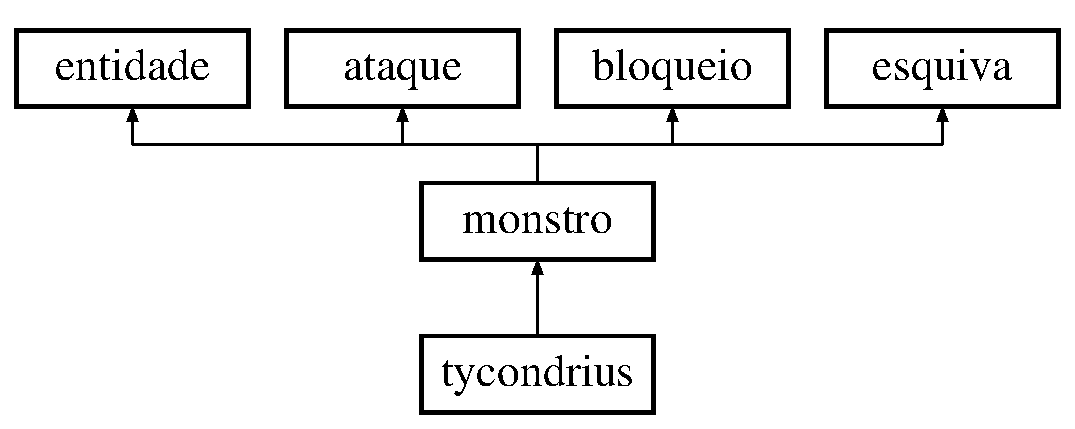
\includegraphics[height=3.000000cm]{classtycondrius}
\end{center}
\end{figure}
\subsection*{Public Member Functions}
\begin{DoxyCompactItemize}
\item 
\mbox{\hyperlink{classtycondrius_abc367b8da7d7d6d0709be8e76b911bf2}{tycondrius}} ()
\begin{DoxyCompactList}\small\item\em Criação da classe tycondrius. \end{DoxyCompactList}\end{DoxyCompactItemize}


\subsection{Constructor \& Destructor Documentation}
\mbox{\Hypertarget{classtycondrius_abc367b8da7d7d6d0709be8e76b911bf2}\label{classtycondrius_abc367b8da7d7d6d0709be8e76b911bf2}} 
\index{tycondrius@{tycondrius}!tycondrius@{tycondrius}}
\index{tycondrius@{tycondrius}!tycondrius@{tycondrius}}
\subsubsection{\texorpdfstring{tycondrius()}{tycondrius()}}
{\footnotesize\ttfamily tycondrius\+::tycondrius (\begin{DoxyParamCaption}{ }\end{DoxyParamCaption})}



Criação da classe tycondrius. 

Utilização da classe monstro como base. \begin{DoxyReturn}{Returns}
Objeto tycondrius. 
\end{DoxyReturn}


The documentation for this class was generated from the following files\+:\begin{DoxyCompactItemize}
\item 
tycondrius.\+h\item 
tycondrius.\+cpp\end{DoxyCompactItemize}

\hypertarget{classverdugo}{}\section{verdugo Class Reference}
\label{classverdugo}\index{verdugo@{verdugo}}
Inheritance diagram for verdugo\+:\begin{figure}[H]
\begin{center}
\leavevmode
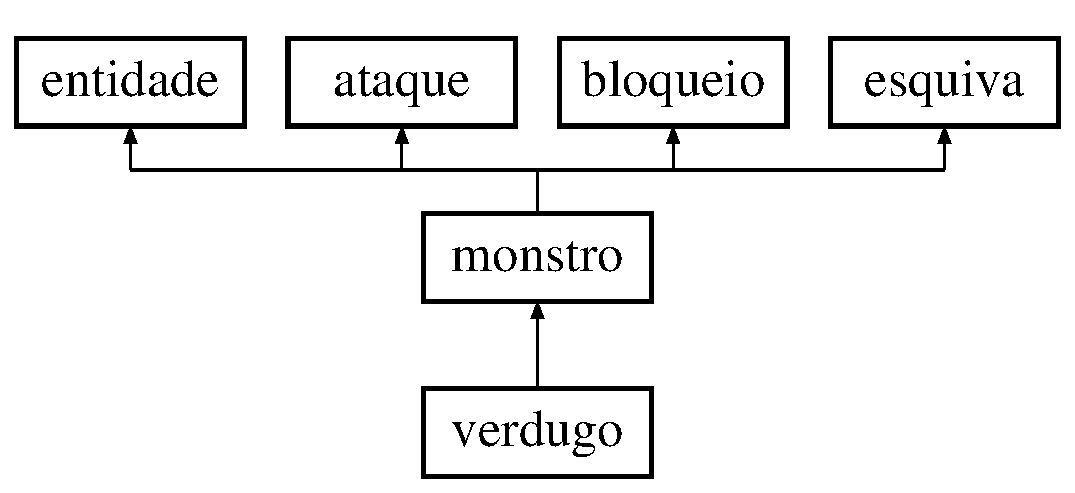
\includegraphics[height=3.000000cm]{classverdugo}
\end{center}
\end{figure}
\subsection*{Public Member Functions}
\begin{DoxyCompactItemize}
\item 
\mbox{\hyperlink{classverdugo_aa7b5dc56ccf1f758fb7cec5b6b7306ab}{verdugo}} ()
\begin{DoxyCompactList}\small\item\em Criação da classe verdugo. \end{DoxyCompactList}\end{DoxyCompactItemize}


\subsection{Constructor \& Destructor Documentation}
\mbox{\Hypertarget{classverdugo_aa7b5dc56ccf1f758fb7cec5b6b7306ab}\label{classverdugo_aa7b5dc56ccf1f758fb7cec5b6b7306ab}} 
\index{verdugo@{verdugo}!verdugo@{verdugo}}
\index{verdugo@{verdugo}!verdugo@{verdugo}}
\subsubsection{\texorpdfstring{verdugo()}{verdugo()}}
{\footnotesize\ttfamily verdugo\+::verdugo (\begin{DoxyParamCaption}{ }\end{DoxyParamCaption})}



Criação da classe verdugo. 

Utilização da classe monstro como base. \begin{DoxyReturn}{Returns}
Objeto verdugo. 
\end{DoxyReturn}


The documentation for this class was generated from the following files\+:\begin{DoxyCompactItemize}
\item 
verdugo.\+h\item 
verdugo.\+cpp\end{DoxyCompactItemize}

\hypertarget{classviking}{}\section{viking Class Reference}
\label{classviking}\index{viking@{viking}}
Inheritance diagram for viking\+:\begin{figure}[H]
\begin{center}
\leavevmode
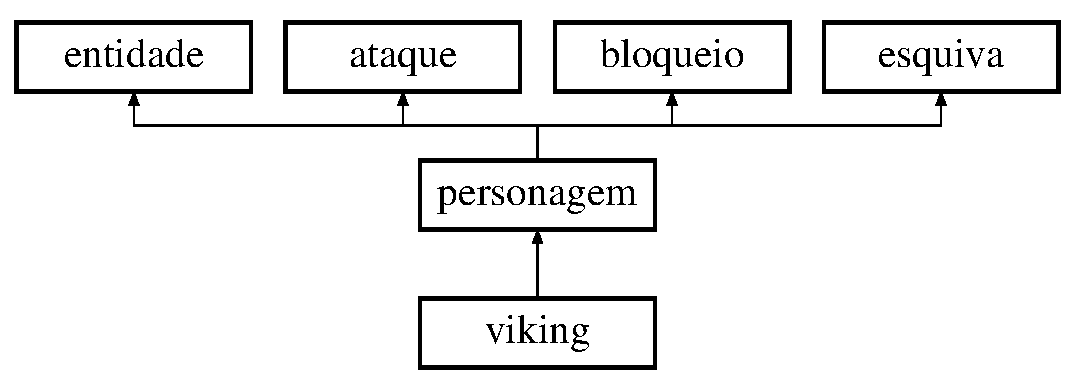
\includegraphics[height=3.000000cm]{classviking}
\end{center}
\end{figure}
\subsection*{Public Member Functions}
\begin{DoxyCompactItemize}
\item 
\mbox{\hyperlink{classviking_aec7e94a062284984afac0ffc49ea5213}{viking}} (string nome)
\begin{DoxyCompactList}\small\item\em Criação da classe viking. \end{DoxyCompactList}\item 
int \mbox{\hyperlink{classviking_aba7bbd831d9b38d98b74ca805d2ea250}{controle\+Ataque}} (string valor, int arm\+Fisica, int arm\+Runica, int hp)
\begin{DoxyCompactList}\small\item\em Método de controle de ataque. \end{DoxyCompactList}\item 
int \mbox{\hyperlink{classviking_a433998767ad855cbfa152c1b0f32363e}{skill\+Um}} (int arm\+Fisica, int arm\+Runica, int hp)
\begin{DoxyCompactList}\small\item\em Método skill\+Um. \end{DoxyCompactList}\item 
int \mbox{\hyperlink{classviking_a5d9d645dae5e647b668c57afa0be1cd8}{skill\+Dois}} (int arm\+Fisica, int arm\+Runica, int hp)
\begin{DoxyCompactList}\small\item\em Método skill\+Dois. \end{DoxyCompactList}\item 
int \mbox{\hyperlink{classviking_a68c634c68c727ebd2638965b6d393f42}{skill\+Tres}} (int arm\+Fisica, int arm\+Runica, int hp)
<<<<<<< HEAD
\begin{DoxyCompactList}\small\item\em Método skill\+Um. \end{DoxyCompactList}\item 
void \mbox{\hyperlink{classviking_a486735595f8a0f86a075699bec76c03e}{help}} ()
\begin{DoxyCompactList}\small\item\em Método help. \end{DoxyCompactList}\end{DoxyCompactItemize}
=======
\begin{DoxyCompactList}\small\item\em Método skill\+Um. \end{DoxyCompactList}\end{DoxyCompactItemize}
>>>>>>> 0546f94c50e08ebf892bc8350edb40cb6ecd7634


\subsection{Constructor \& Destructor Documentation}
\mbox{\Hypertarget{classviking_aec7e94a062284984afac0ffc49ea5213}\label{classviking_aec7e94a062284984afac0ffc49ea5213}} 
\index{viking@{viking}!viking@{viking}}
\index{viking@{viking}!viking@{viking}}
\subsubsection{\texorpdfstring{viking()}{viking()}}
{\footnotesize\ttfamily viking\+::viking (\begin{DoxyParamCaption}\item[{string}]{Nome }\end{DoxyParamCaption})}



Criação da classe viking. 

Utilização da classe personagem como base. \begin{DoxyReturn}{Returns}
Objeto viking. 
\end{DoxyReturn}


\subsection{Member Function Documentation}
\mbox{\Hypertarget{classviking_aba7bbd831d9b38d98b74ca805d2ea250}\label{classviking_aba7bbd831d9b38d98b74ca805d2ea250}} 
\index{viking@{viking}!controle\+Ataque@{controle\+Ataque}}
\index{controle\+Ataque@{controle\+Ataque}!viking@{viking}}
\subsubsection{\texorpdfstring{controle\+Ataque()}{controleAtaque()}}
{\footnotesize\ttfamily int viking\+::controle\+Ataque (\begin{DoxyParamCaption}\item[{string}]{valor,  }\item[{int}]{arm\+Fisica,  }\item[{int}]{arm\+Runica,  }\item[{int}]{hp }\end{DoxyParamCaption})}



Método de controle de ataque. 

recebe valor do usuário, armadura física, armadura mágica e hp do alvo. \begin{DoxyReturn}{Returns}
dano causado. 
\end{DoxyReturn}
<<<<<<< HEAD
\mbox{\Hypertarget{classviking_a486735595f8a0f86a075699bec76c03e}\label{classviking_a486735595f8a0f86a075699bec76c03e}} 
\index{viking@{viking}!help@{help}}
\index{help@{help}!viking@{viking}}
\subsubsection{\texorpdfstring{help()}{help()}}
{\footnotesize\ttfamily void viking\+::help (\begin{DoxyParamCaption}{ }\end{DoxyParamCaption})}



Método help. 

Informa ao jogador detalhes das skills. \begin{DoxyReturn}{Returns}
void. 
\end{DoxyReturn}
=======
>>>>>>> 0546f94c50e08ebf892bc8350edb40cb6ecd7634
\mbox{\Hypertarget{classviking_a5d9d645dae5e647b668c57afa0be1cd8}\label{classviking_a5d9d645dae5e647b668c57afa0be1cd8}} 
\index{viking@{viking}!skill\+Dois@{skill\+Dois}}
\index{skill\+Dois@{skill\+Dois}!viking@{viking}}
\subsubsection{\texorpdfstring{skill\+Dois()}{skillDois()}}
{\footnotesize\ttfamily int viking\+::skill\+Dois (\begin{DoxyParamCaption}\item[{int}]{arm\+Fisica,  }\item[{int}]{arm\+Runica,  }\item[{int}]{hp }\end{DoxyParamCaption})}



Método skill\+Dois. 

Dano baseado na armadura física, custo de 30 de hp. \begin{DoxyReturn}{Returns}
Dano causado. 
\end{DoxyReturn}
\mbox{\Hypertarget{classviking_a68c634c68c727ebd2638965b6d393f42}\label{classviking_a68c634c68c727ebd2638965b6d393f42}} 
\index{viking@{viking}!skill\+Tres@{skill\+Tres}}
\index{skill\+Tres@{skill\+Tres}!viking@{viking}}
\subsubsection{\texorpdfstring{skill\+Tres()}{skillTres()}}
{\footnotesize\ttfamily int viking\+::skill\+Tres (\begin{DoxyParamCaption}\item[{int}]{arm\+Fisica,  }\item[{int}]{arm\+Runica,  }\item[{int}]{hp }\end{DoxyParamCaption})}



Método skill\+Um. 

Dano que se acertar mata instantâneamente o alvo, custa 150 de hp. \begin{DoxyReturn}{Returns}
Dano causado. 
\end{DoxyReturn}
\mbox{\Hypertarget{classviking_a433998767ad855cbfa152c1b0f32363e}\label{classviking_a433998767ad855cbfa152c1b0f32363e}} 
\index{viking@{viking}!skill\+Um@{skill\+Um}}
\index{skill\+Um@{skill\+Um}!viking@{viking}}
\subsubsection{\texorpdfstring{skill\+Um()}{skillUm()}}
{\footnotesize\ttfamily int viking\+::skill\+Um (\begin{DoxyParamCaption}\item[{int}]{arm\+Fisica,  }\item[{int}]{arm\+Runica,  }\item[{int}]{hp }\end{DoxyParamCaption})}



Método skill\+Um. 

Dano fixo de 35, custo de mana 5. \begin{DoxyReturn}{Returns}
Dano causado. 
\end{DoxyReturn}


The documentation for this class was generated from the following files\+:\begin{DoxyCompactItemize}
\item 
viking.\+h\item 
viking.\+cpp\end{DoxyCompactItemize}

%--- End generated contents ---

% Index
\backmatter
\newpage
\phantomsection
\clearemptydoublepage
\addcontentsline{toc}{chapter}{\indexname}
\printindex

\end{document}
